\chapter{Open Science Framework}\label{appendix:osf}
\thispagestyle{chapterBeginStyle}
\label{appendix:source-code}

Source code is available at \url{https://github.com/burnpiro/xai-correlation}. Repository includes detailed instruction on how to run and reproduce experiments. The source code has an additional Wiki page available at \url{https://github.com/burnpiro/xai-correlation/wiki} with some of the results, links to trained models and additional instructions.

\subsection*{Requirements}

\begin{itemize}
  \item Python 3.8
  \item git
  \item Graphic card with at least 11GB of free memory (tested on GForce GTX 1080Ti)
\end{itemize}

\section{Datasets}\label{appendix:datasets}

\subsection{Stanford Dogs}\label{appendix:datasets:stanford-dogs}

\begin{figure}[ht]
  \centering
 \begin{subfigure}{.48\textwidth}
    \centering
    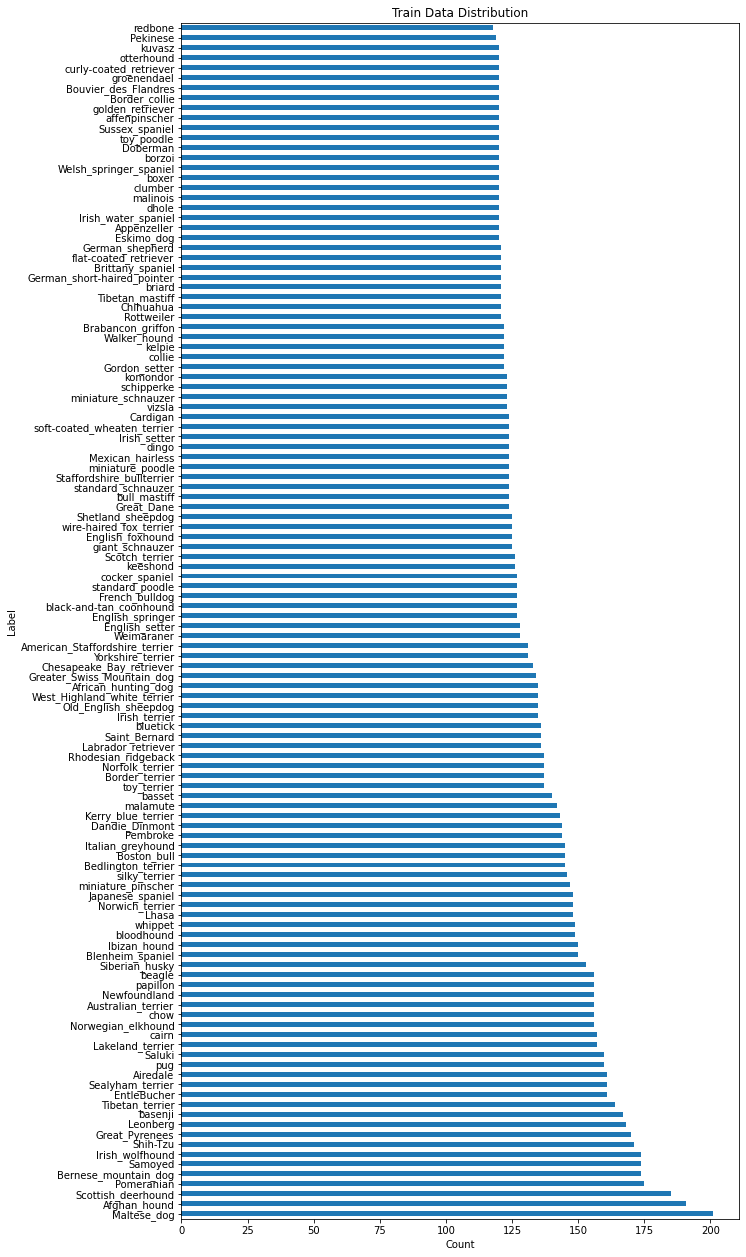
\includegraphics[width=\textwidth]{appendixes/images/dogs-train.png}
    \caption{Train dataset}
\end{subfigure}
 \begin{subfigure}{.48\textwidth}
    \centering
    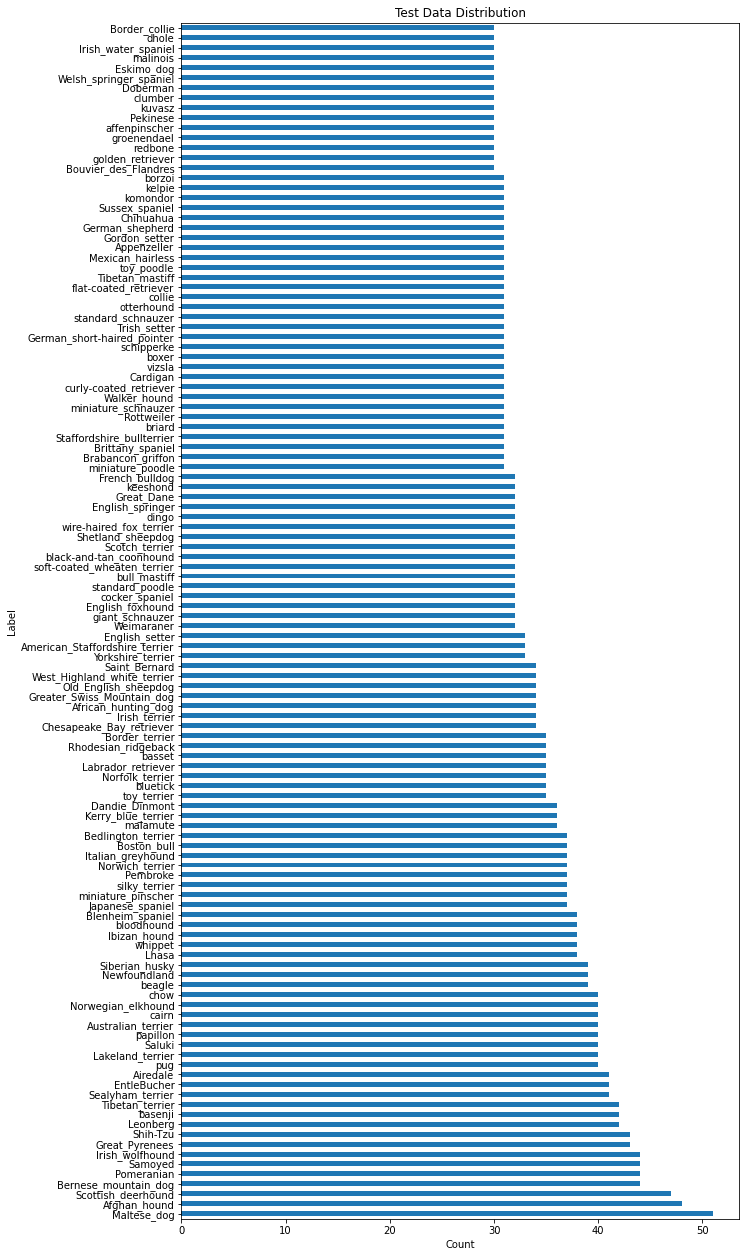
\includegraphics[width=\textwidth]{appendixes/images/dogs-test.png}
    \caption{Test dataset}
\end{subfigure}

 \caption{Class distribution in \textit{Stanford Dogs}\cite{stanford-dogs} dataset. Data available at \url{http://vision.stanford.edu/aditya86/ImageNetDogs/}.}
\end{figure}

\FloatBarrier

\subsection{Food 101}\label{appendix:datasets:food101}

Data available at \url{https://www.kaggle.com/dansbecker/food-101}. Each class has 750 examples in training dataset and 250 examples in test dataset. 101 classes in total.

\FloatBarrier

\subsection{Edible wild plants}\label{appendix:datasets:edible-plants}

\begin{figure}[ht]
  \centering
 \begin{subfigure}{.48\textwidth}
    \centering
    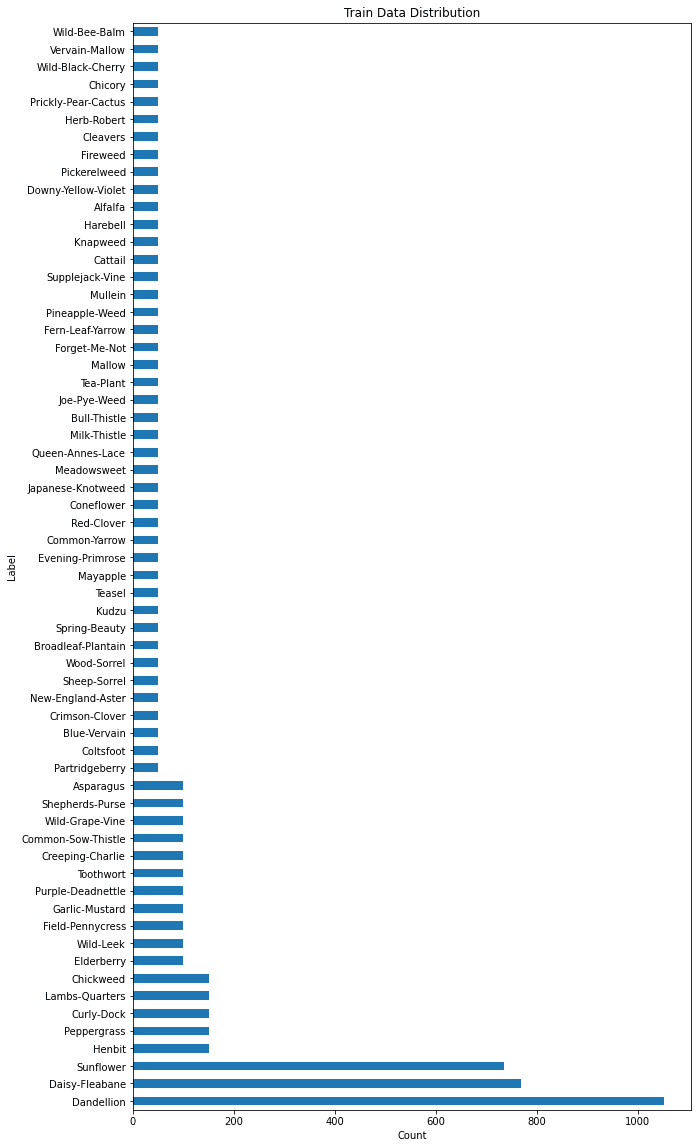
\includegraphics[width=\textwidth]{appendixes/images/edible-train.png}
    \caption{Train dataset}
\end{subfigure}
 \begin{subfigure}{.48\textwidth}
    \centering
    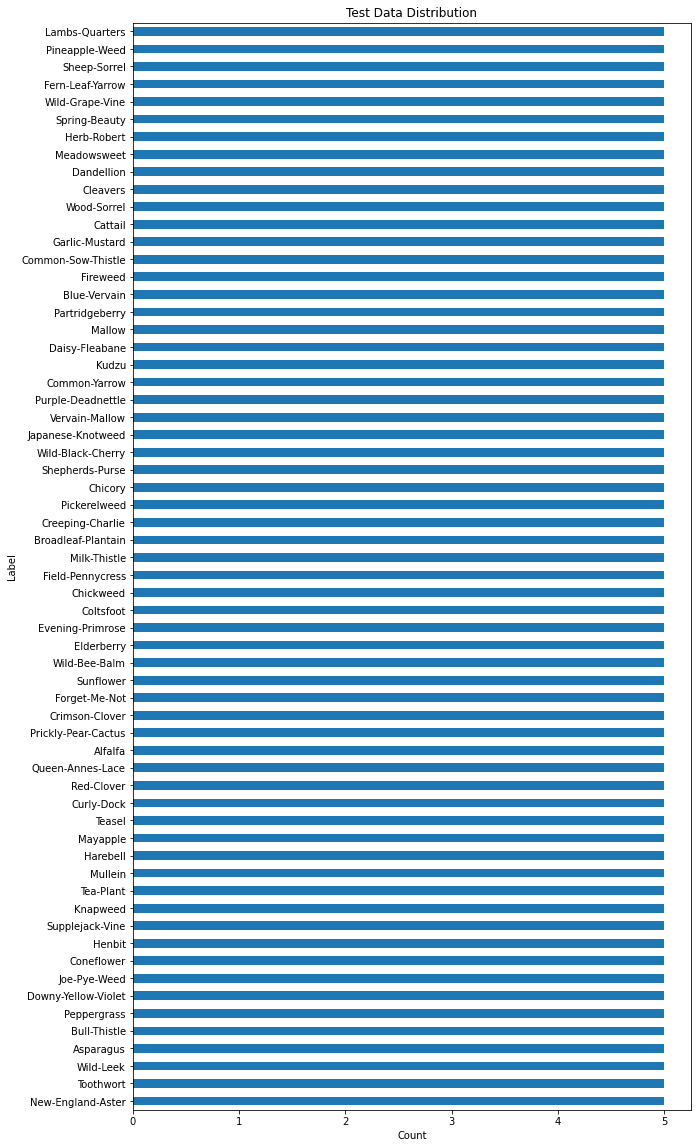
\includegraphics[width=\textwidth]{appendixes/images/edible-test.png}
    \caption{Test dataset}
\end{subfigure}

 \caption{Class distribution in \textit{Edible wild plants}\cite{edible-wild-plants} dataset. Data available at \url{https://www.kaggle.com/gverzea/edible-wild-plants}.}
\end{figure}

\FloatBarrier

\subsection{Marvel Heroes}\label{appendix:datasets:marvel}

\begin{figure}[hbt!]
  \centering
 \begin{subfigure}{.35\textwidth}
    \centering
    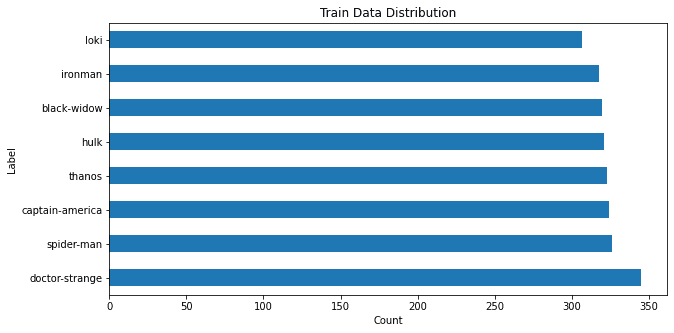
\includegraphics[width=\textwidth]{appendixes/images/marvel-train.png}
    \caption{Train dataset}
\end{subfigure}
 \begin{subfigure}{.35\textwidth}
    \centering
    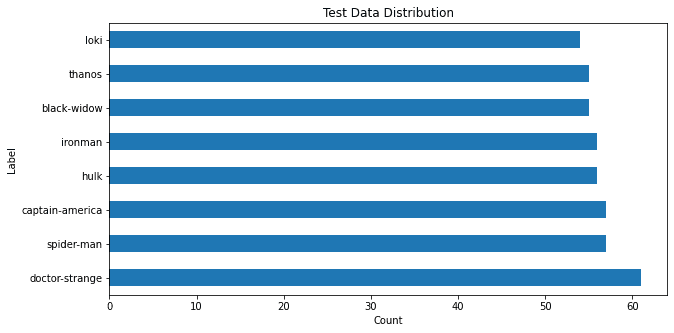
\includegraphics[width=\textwidth]{appendixes/images/marvel-test.png}
    \caption{Test dataset}
\end{subfigure}

 \caption{Class distribution in \textit{Marvel Heroes}\cite{marvel-heroes} dataset. Data available at \url{https://www.kaggle.com/hchen13/marvel-heroes}.}
\end{figure}

\FloatBarrier

\subsection{Plants}\label{appendix:datasets:plants}

\begin{figure}[ht]
  \centering
 \begin{subfigure}{.4\textwidth}
    \centering
    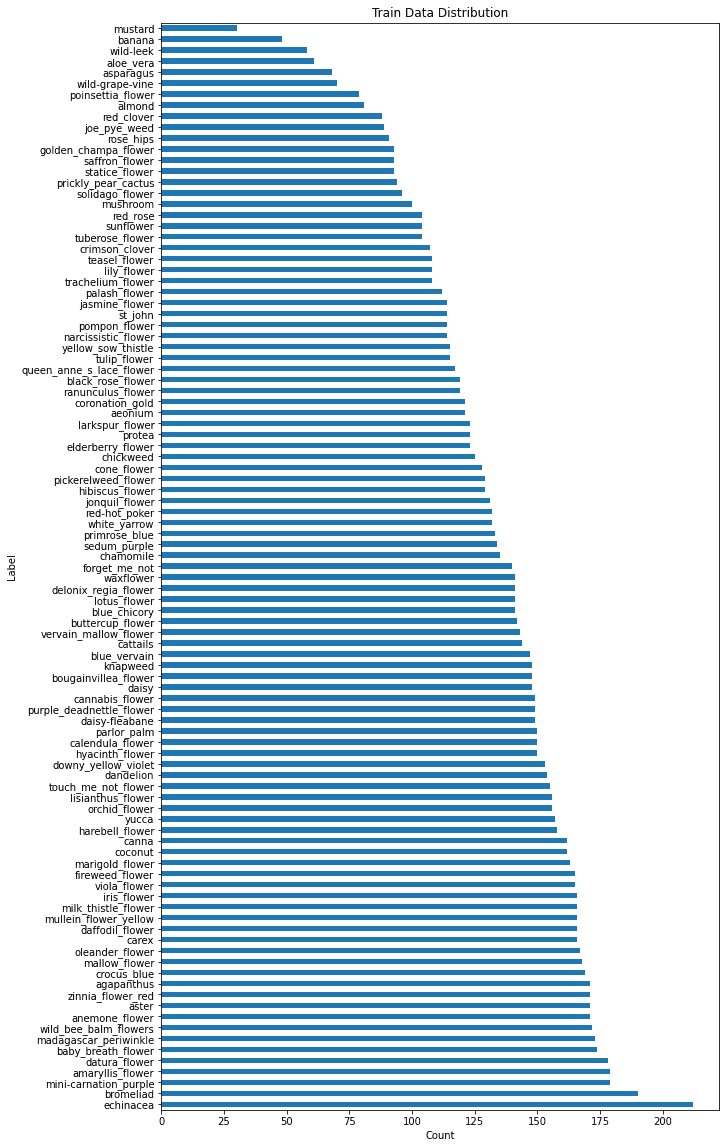
\includegraphics[width=\textwidth]{appendixes/images/plants-train.png}
    \caption{Train dataset}
\end{subfigure}
 \begin{subfigure}{.4\textwidth}
    \centering
    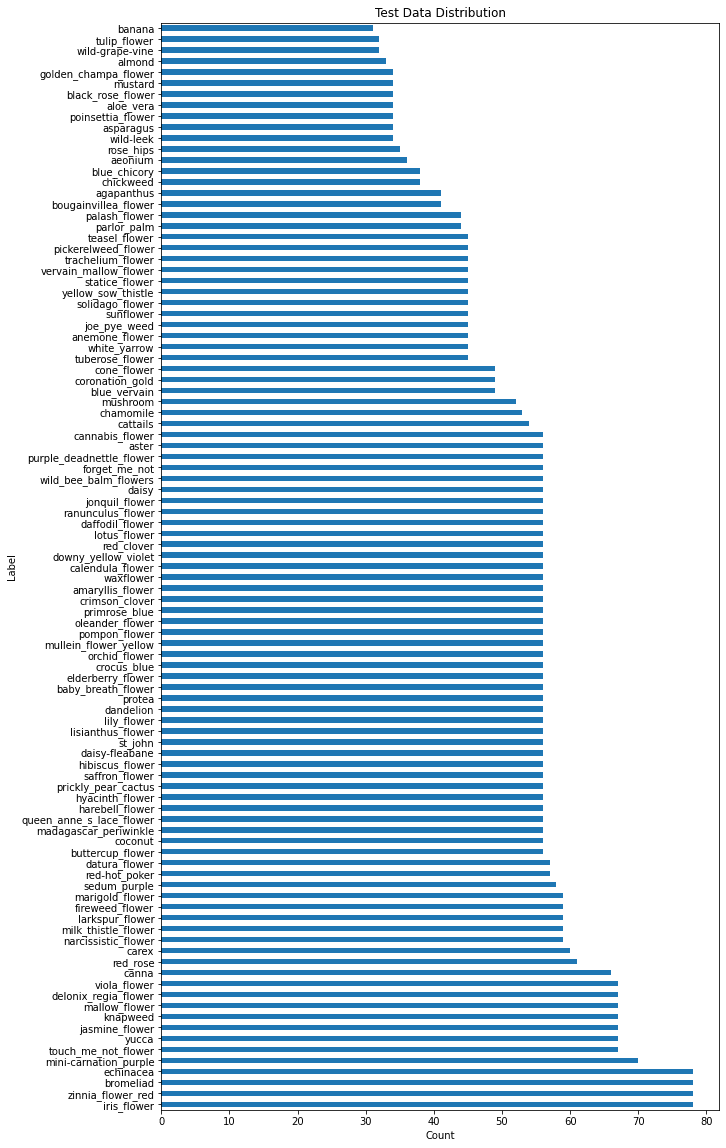
\includegraphics[width=\textwidth]{appendixes/images/plants-test.png}
    \caption{Test dataset}
\end{subfigure}

 \caption{Class distribution in \textit{Plants}\cite{plants-dataset} dataset. Data available at \url{https://www.kaggle.com/muhammadjawad1998/plants-dataset99-classes?select=Plant_Data}.}
\end{figure}

\FloatBarrier

\section{Models}\label{appendix:models:scores}

Trained models are available at \url{https://drive.google.com/drive/folders/1WVmokp5vaPwOGhpEC6elGVE0aM7fPqNU?usp=sharing}. Step by step instruction on how to train models is available at \url{https://github.com/burnpiro/xai-correlation/wiki/Train-and-Eval-Models}.

\begin{longtable}{|l|l|l|l|r|r|}
\caption{Models' F1 and Accuracy scores}
\label{tab:appendix:models:all-scores} \\\hline
ID &        Dataset &         Model & Data Fraction &     Acc &      F1 \\\hline
0  &  Edible wild plants &      ResNet18 &       100\% &  0.8146 &  0.7671 \\
1  &  Edible wild plants &      ResNet18 &        80\% &  0.7867 &  0.7348 \\
2  &  Edible wild plants &      ResNet18 &        60\% &  0.7709 &  0.7168 \\
3  &  Edible wild plants &      ResNet18 &        40\% &  0.7411 &  0.6634 \\
4  &  Edible wild plants &      ResNet18 &        20\% &  0.5519 &  0.4914 \\\hline
5  &        Food101 &      ResNet18 &       100\% &  0.7650 &  0.7632 \\
6  &        Food101 &      ResNet18 &        80\% &  0.7550 &  0.7532 \\
7  &        Food101 &      ResNet18 &        60\% &  0.7362 &  0.7326 \\
8  &        Food101 &      ResNet18 &        40\% &  0.7146 &  0.7122 \\
9  &        Food101 &      ResNet18 &        20\% &  0.6741 &  0.6689 \\\hline
10 &         Marvel Heroes &      ResNet18 &       100\% &  0.6813 &  0.6798 \\
11 &         Marvel Heroes &      ResNet18 &        80\% &  0.6935 &  0.6923 \\
12 &         Marvel Heroes &      ResNet18 &        60\% &  0.6759 &  0.6693 \\
13 &         Marvel Heroes &      ResNet18 &        40\% &  0.6361 &  0.6301 \\
14 &         Marvel Heroes &      ResNet18 &        20\% &  0.6017 &  0.5960 \\\hline
15 &     Plants &      ResNet18 &       100\% &  0.8895 &  0.8860 \\
16 &     Plants &      ResNet18 &        80\% &  0.8648 &  0.8590 \\
17 &     Plants &      ResNet18 &        60\% &  0.8287 &  0.8240 \\
18 &     Plants &      ResNet18 &        40\% &  0.7912 &  0.7855 \\
19 &     Plants &      ResNet18 &        20\% &  0.7189 &  0.7010 \\\hline
20 &  Stanford Dogs &      ResNet18 &       100\% &  0.7738 &  0.7662 \\
21 &  Stanford Dogs &      ResNet18 &        80\% &  0.7757 &  0.7681 \\
22 &  Stanford Dogs &      ResNet18 &        60\% &  0.7676 &  0.7618 \\
23 &  Stanford Dogs &      ResNet18 &        40\% &  0.7633 &  0.7567 \\
24 &  Stanford Dogs &      ResNet18 &        20\% &  0.7278 &  0.7208 \\\hline
25 &  Edible wild plants &  EfficientNet B0 &       100\% &  0.8067 &  0.7359 \\
26 &  Edible wild plants &  EfficientNet B0 &        80\% &  0.7805 &  0.7253 \\
27 &  Edible wild plants &  EfficientNet B0 &        60\% &  0.7165 &  0.6338 \\
28 &  Edible wild plants &  EfficientNet B0 &        40\% &  0.5760 &  0.5312 \\
29 &  Edible wild plants &  EfficientNet B0 &        20\% &  0.3392 &  0.2713 \\\hline
30 &        Food101 &  EfficientNet B0 &       100\% &  0.8374 &  0.8368 \\
31 &        Food101 &  EfficientNet B0 &        80\% &  0.8253 &  0.8248 \\
32 &        Food101 &  EfficientNet B0 &        60\% &  0.8140 &  0.8131 \\
33 &        Food101 &  EfficientNet B0 &        40\% &  0.7871 &  0.7870 \\
34 &        Food101 &  EfficientNet B0 &        20\% &  0.7395 &  0.7385 \\\hline
35 &         Marvel Heroes &  EfficientNet B0 &       100\% &  0.7119 &  0.7041 \\
36 &         Marvel Heroes &  EfficientNet B0 &        80\% &  0.6918 &  0.6831 \\
37 &         Marvel Heroes &  EfficientNet B0 &        60\% &  0.6892 &  0.6856 \\
38 &         Marvel Heroes &  EfficientNet B0 &        40\% &  0.6493 &  0.6444 \\
39 &         Marvel Heroes &  EfficientNet B0 &        20\% &  0.5831 &  0.5774 \\\hline
40 &     Plants &  EfficientNet B0 &       100\% &  0.8734 &  0.8703 \\
41 &     Plants &  EfficientNet B0 &        80\% &  0.8523 &  0.8487 \\
42 &     Plants &  EfficientNet B0 &        60\% &  0.8218 &  0.8165 \\
43 &     Plants &  EfficientNet B0 &        40\% &  0.7774 &  0.7664 \\
44 &     Plants &  EfficientNet B0 &        20\% &  0.6734 &  0.6422 \\\hline
45 &  Stanford Dogs &  EfficientNet B0 &       100\% &  0.8343 &  0.8289 \\
46 &  Stanford Dogs &  EfficientNet B0 &        80\% &  0.8293 &  0.8253 \\
47 &  Stanford Dogs &  EfficientNet B0 &        60\% &  0.8240 &  0.8187 \\
48 &  Stanford Dogs &  EfficientNet B0 &        40\% &  0.8041 &  0.7972 \\
49 &  Stanford Dogs &  EfficientNet B0 &        20\% &  0.7654 &  0.7549 \\\hline
50 &  Edible wild plants &      DenseNet 121 &       100\% &  0.8777 &  0.8357 \\
51 &  Edible wild plants &      DenseNet 121 &        80\% &  0.8520 &  0.8145 \\
52 &  Edible wild plants &      DenseNet 121 &        60\% &  0.8062 &  0.7502 \\
53 &  Edible wild plants &      DenseNet 121 &        40\% &  0.7718 &  0.7210 \\
54 &  Edible wild plants &      DenseNet 121 &        20\% &  0.6576 &  0.5957 \\\hline
55 &        Food101 &      DenseNet 121 &       100\% &  0.8465 &  0.8447 \\
56 &        Food101 &      DenseNet 121 &        80\% &  0.8356 &  0.8346 \\
57 &        Food101 &      DenseNet 121 &        60\% &  0.8213 &  0.8189 \\
58 &        Food101 &      DenseNet 121 &        40\% &  0.8023 &  0.8005 \\
59 &        Food101 &      DenseNet 121 &        20\% &  0.7585 &  0.7555 \\\hline
60 &         Marvel Heroes &      DenseNet 121 &       100\% &  0.7196 &  0.7127 \\
61 &         Marvel Heroes &      DenseNet 121 &        80\% &  0.6919 &  0.6911 \\
62 &         Marvel Heroes &      DenseNet 121 &        60\% &  0.7164 &  0.7101 \\
63 &         Marvel Heroes &      DenseNet 121 &        40\% &  0.6853 &  0.6739 \\
64 &         Marvel Heroes &      DenseNet 121 &        20\% &  0.6777 &  0.6582 \\\hline
65 &     Plants &      DenseNet 121 &       100\% &  0.9016 &  0.8995 \\
66 &     Plants &      DenseNet 121 &        80\% &  0.8829 &  0.8799 \\
67 &     Plants &      DenseNet 121 &        60\% &  0.8567 &  0.8516 \\
68 &     Plants &      DenseNet 121 &        40\% &  0.8233 &  0.8182 \\
69 &     Plants &      DenseNet 121 &        20\% &  0.7494 &  0.7397 \\\hline
70 &  Stanford Dogs &      DenseNet 121 &       100\% &  0.8290 &  0.8244 \\
71 &  Stanford Dogs &      DenseNet 121 &        80\% &  0.8179 &  0.8130 \\
72 &  Stanford Dogs &      DenseNet 121 &        60\% &  0.8153 &  0.8099 \\
73 &  Stanford Dogs &      DenseNet 121 &        40\% &  0.8042 &  0.7989 \\
74 &  Stanford Dogs &      DenseNet 121 &        20\% &  0.7932 &  0.7846 \\\hline
\end{longtable}

\chapter{Supplementary Results}\label{appendix:supplementary}
\thispagestyle{chapterBeginStyle}
\label{appendix:supplementary-results}

\section{Don't Augment Me - appendix}\label{appendix:dont-augment}

\subsection{SSIM attribution ranges}\label{appendix:ssim-ranges}

\begin{table}[h]
 \centering
  \caption{SSIM ranges for attribution methods for ResNet18}
  \label{tab:ranges-for-resnet}
    \begin{tabular}{|l|lllll|}
    \hline
     \backslashbox{Attribution}{Dataset} & Edible plants & Food 101 & Marvel & Plants &
     Stanford Dogs \\
     \hline
    Deconvolution & 0.784622 & 0.423285 & 0.473029 & 0.682504 & 1.283490\\
    Integrated Gradients & 0.421971 & 1.306827 & 0.611498 & 0.887589 & 1.565911\\
    Saliency & 0.047666 & 0.045500 & 0.067406 & 0.094456 & 0.060711\\
    Grad-Cam  & 0.000047 & 0.000051 & 0.000022 & 0.000085 & 0.000064 \\
    Grad-Shap & 0.145404 & 0.093035 & 0.102947 & 0.285072 & 0.147860 \\
    Guided Backprop & 0.079774 & 0.069185 & 0.050991 & 0.126553 & 0.152545 \\
    \hline
    \end{tabular}
\end{table}


\begin{table}[h]
 \centering
  \caption{SSIM ranges for attribution methods for DenseNet121}
  \label{tab:ranges-for-densenet}
    \begin{tabular}{|l|lllll|}
    \hline
     \backslashbox{Attribution}{Dataset} & Edible plants & Food 101 & Marvel & Plants &
     Stanford Dogs \\
     \hline
    Deconvolution & 4677.117 & 80.11916 & 3037.732 & 1715.939 & 2044.188\\
    Integrated Gradients & 1.099644 & 2.577734 & 0.997656 & 0.816421 & 2.090753\\
    Saliency & 0.068720 & 0.048571 & 0.052243 & 0.068942 & 0.149736\\
    Grad-Cam  & 0.000278 & 0.000187 & 0.000510 & 0.000395 & 0.002106 \\
    Grad-Shap & 0.142074 & 0.119778 & 0.162216 & 0.143393 & 0.345822\\
    Guided Backprop & 0.400560 & 0.218944 & 0.512460 & 0.720738 & 1.565153\\
    \hline
    \end{tabular}
\end{table}

\begin{table}[h]
 \centering
  \caption{SSIM ranges for attribution methods for EfficientNet B0}
  \label{tab:ranges-for-efficientnet}
    \begin{tabular}{|l|lllll|}
    \hline
     \backslashbox{Attribution}{Dataset} & Edible plants & Food 101 & Marvel & Plants &
     Stanford Dogs \\
     \hline
    Deconvolution & 0.078107 & 0.025042 & 0.030603 & 0.055335 & 0.071512\\
    Integrated Gradients & 0.732469 & 5.059399 & 0.810054 & 1.551912 & 2.329165\\
    Saliency & 0.095080 & 0.032253 & 0.043658 & 0.140426 & 0.136111\\
    Grad-Cam  & 0.000028 & 0.000005 & 0.000007 & 0.000042 & 0.000037 \\
    Grad-Shap & 0.464270 & 0.054290 & 0.154112 & 0.280005 & 0.352823\\
    Guided Backprop & 0.068730 & 0.037462 & 0.030622 & 0.066075 & 0.102107\\
    \hline
    \end{tabular}
\end{table}

\subsection{Detailed SSIM results}

\begin{figure}[ht]
  \centering
  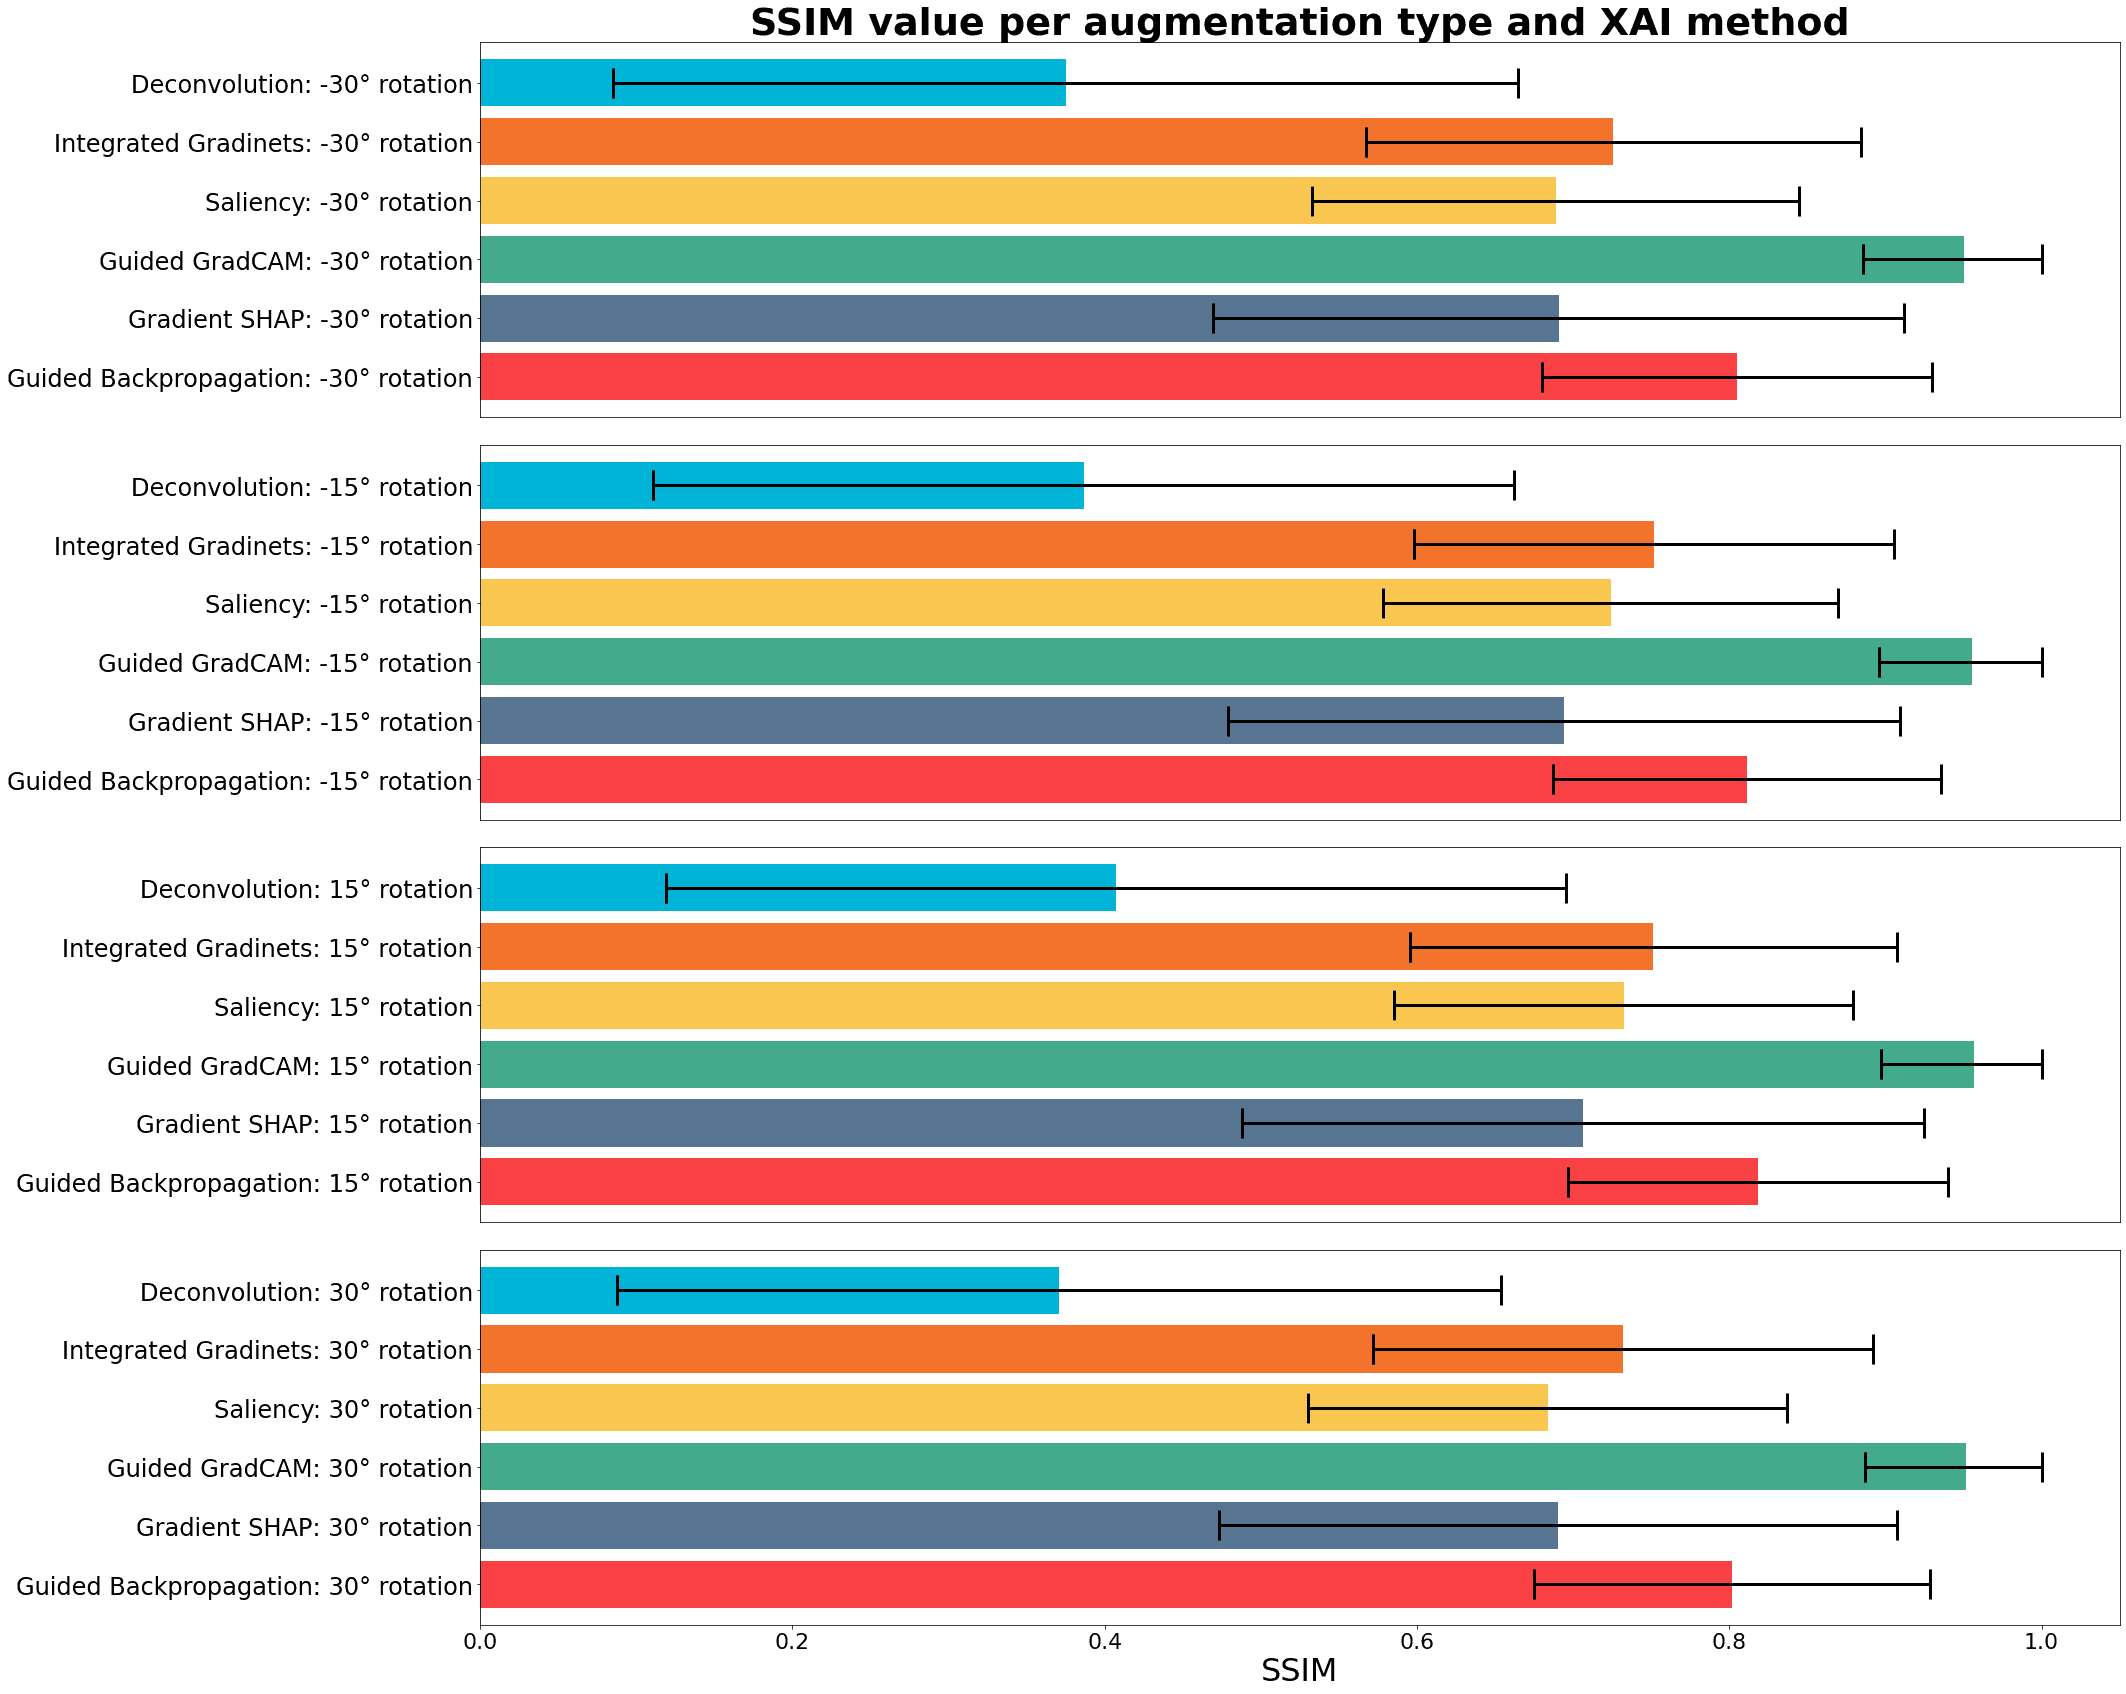
\includegraphics[width=\textwidth]{appendixes/images/rotation-ssim.png}
  \caption{Average SSIM values per attribution method and augmentation type (rotations). Each bar represents a methods' mean value of SSIM. Values used to calculate the mean value are restricted to come only from images augmented by applying specific rotations.}\label{fig:SSIM-all-rotation}
\end{figure}

\begin{figure}[ht]
  \centering
  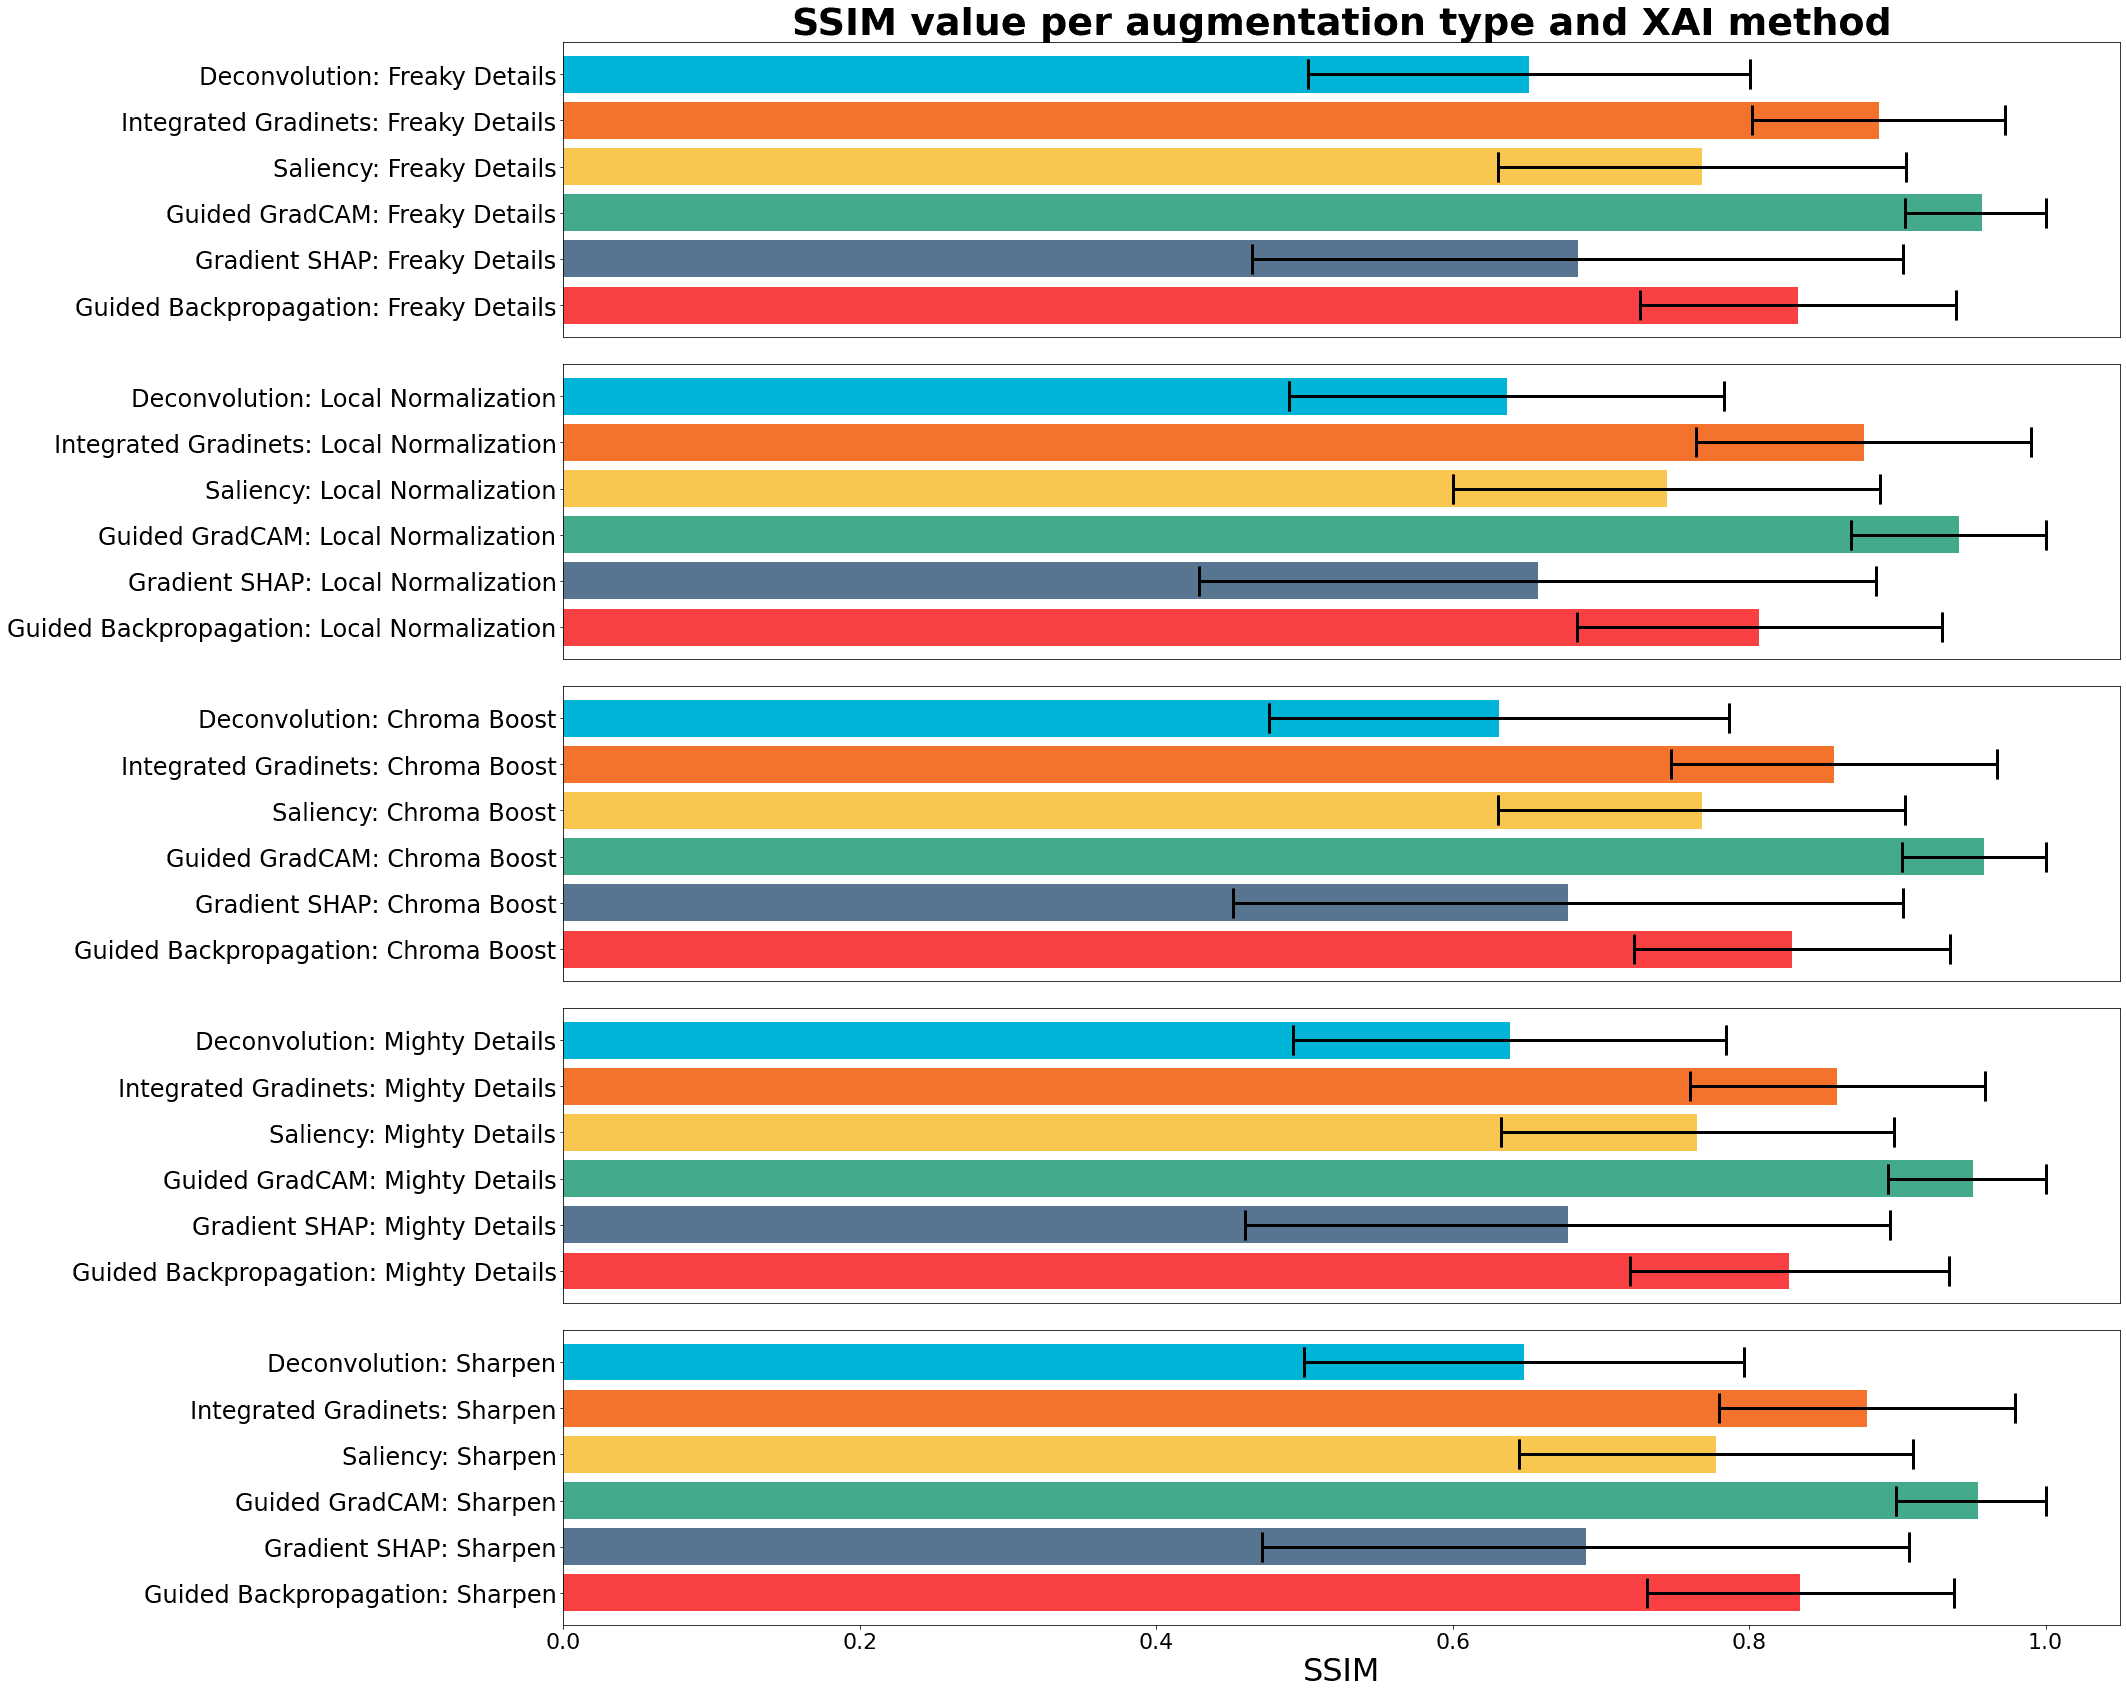
\includegraphics[width=\textwidth]{appendixes/images/filters-ssim.png}
  \caption{Average SSIM values per attribution method and augmentation type (filters). Each bar represents a methods' mean value of SSIM. Values used to calculate the mean value are restricted to come only from images augmented by applying specific filter.}\label{fig:SSIM-all-filters}
\end{figure}

\FloatBarrier

\subsection{Attributions samples}\label{appendix:attribution-samples}

Because the amount of attribution examples is to large to fit them in the appendix, they are available at \url{https://drive.google.com/drive/folders/1Vp3MYRg8j-6ZAfDePeT5kHYPu2Rv6r4t?usp=sharing} (total number of files equals $97990$). File structure is following the pattern \verb|{Augmentation Type}/{Dataset}/{Model version}/{XAI method}|. Each image has a filename containing:

\verb|{index}-{sample id}-{class id}-{augmentation method}-{true class}-{predicted class}.png|

\vspace{5mm}

Combined attribution samples are available at

\url{https://drive.google.com/drive/folders/1lnNQwH3-H1cHiNOEcmnd4OhSScDSuzt0?usp=sharing}.

\begin{figure}[ht]
  \centering
  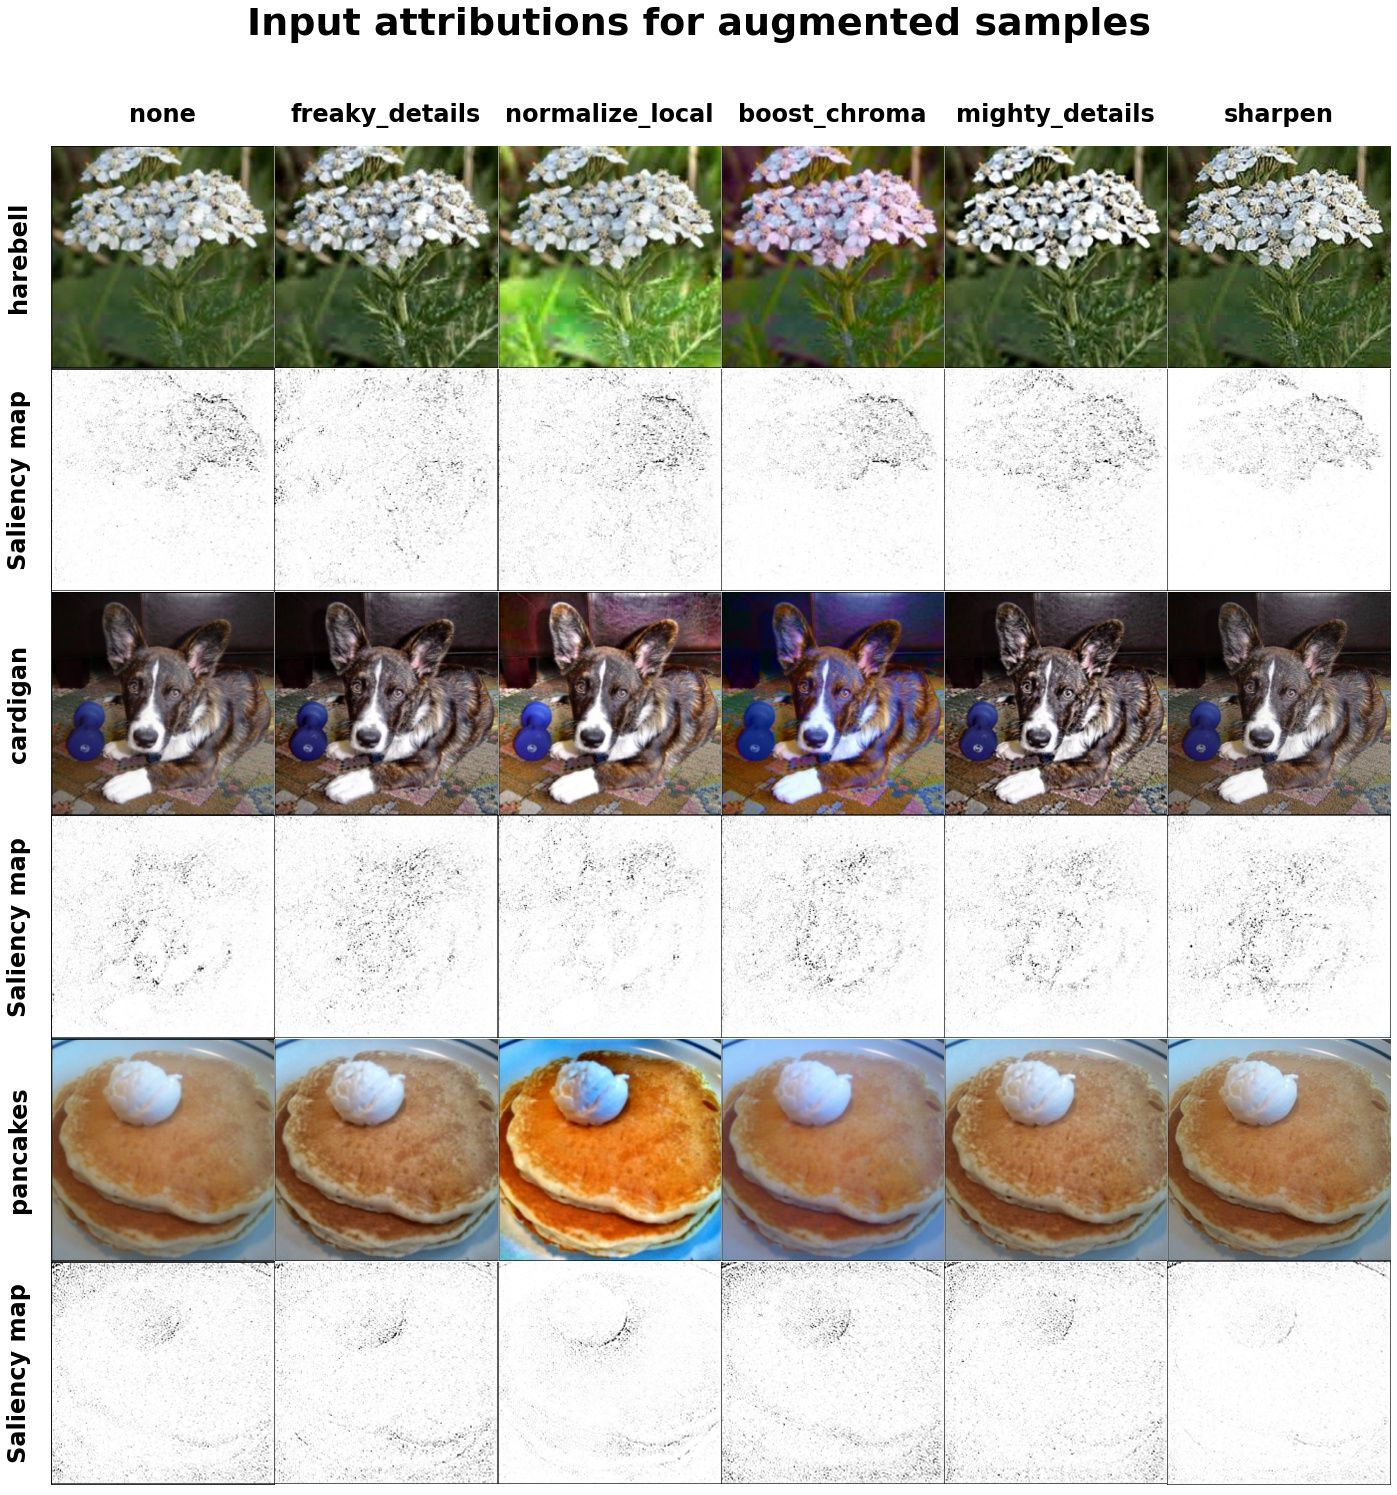
\includegraphics[width=0.8\textwidth]{appendixes/images/filters-sample.jpg}
  \caption{\textbf{Attribution comparison of inputs with applied filters.} Figure shows three distinct images (\textit{harebell\_flower}, \textit{cardigan}, \textit{pancakes}) with different filters. All attributions done by Guided GradCAM.}\label{fig:filters-samples}
\end{figure}

\begin{figure}[ht]
  \centering
  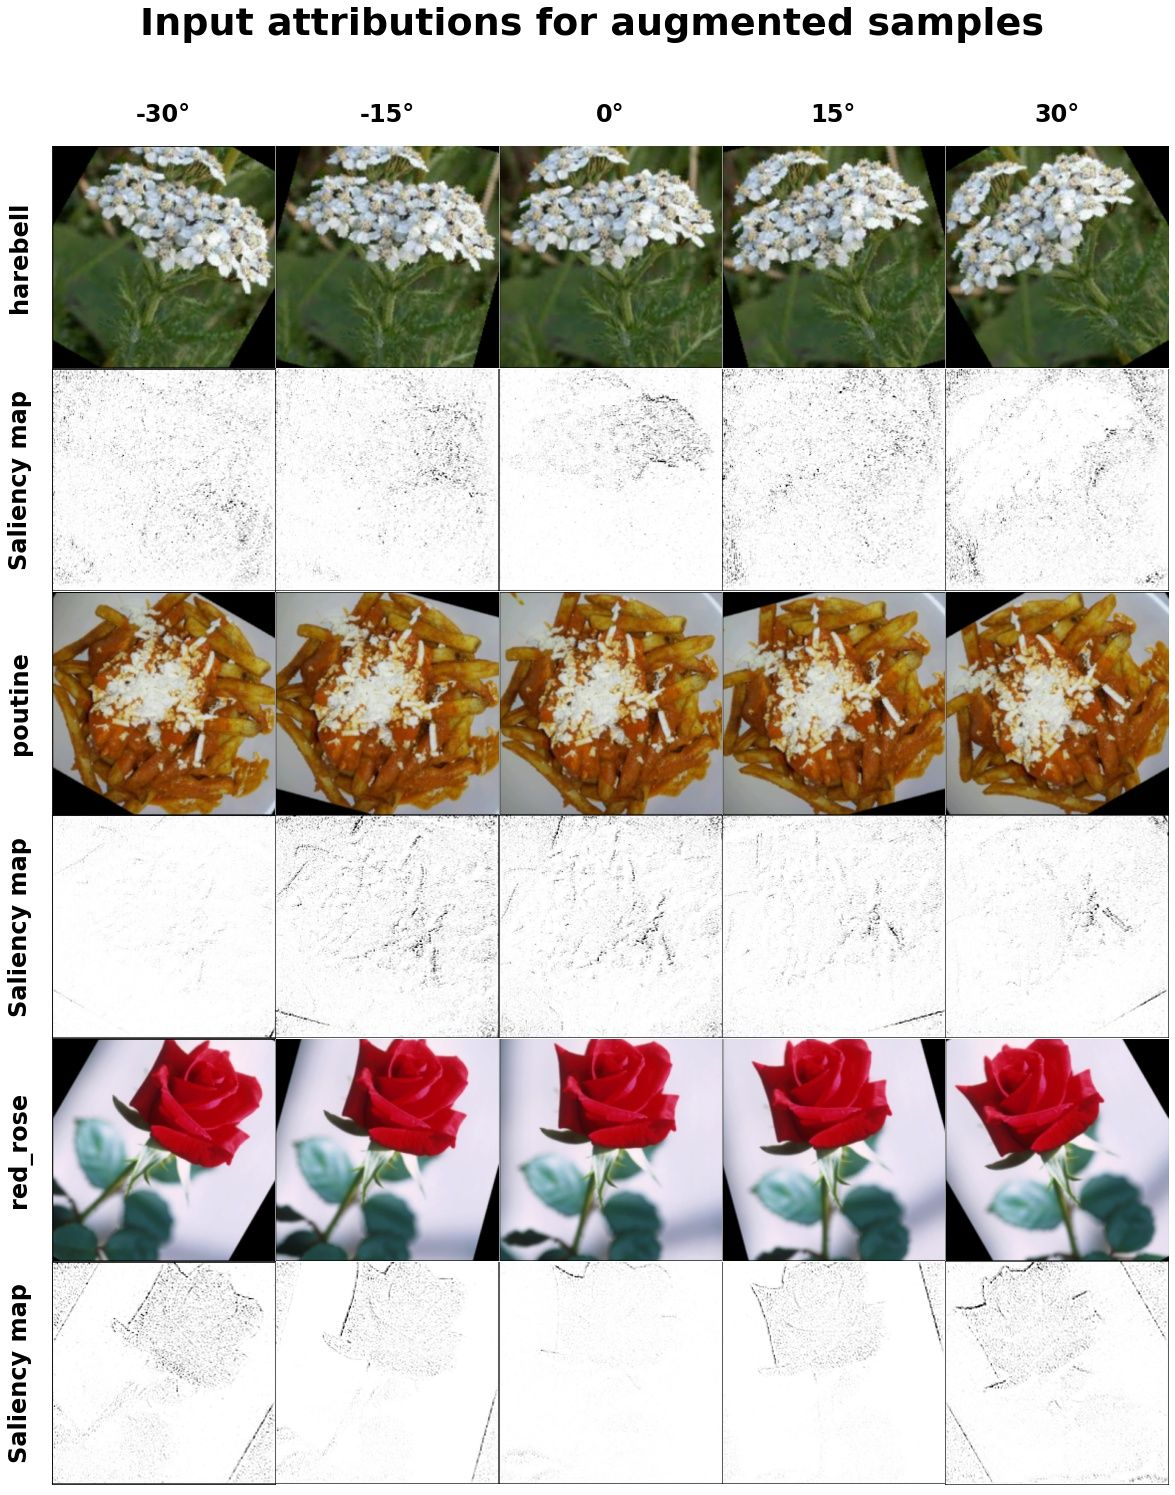
\includegraphics[width=0.8\textwidth]{appendixes/images/rotation-sample.jpg}
  \caption{\textbf{Attribution comparison of rotated inputs.} Figure shows three distinct images (\textit{harebell\_flower}, \textit{poutine}, \textit{red\_rose}) with different rotations. All attributions done by Guided GradCAM.}\label{fig:rotation-samples}
\end{figure}
\section{Can I Rely On You - appendix}\label{appendix:can-i-rely}

\subsection*{Attribution Examples}\label{appendix:attribution-examples}

Because the amount of attribution examples is to large to fit them in the appendix, they are available at \url{https://drive.google.com/drive/folders/177nMz2Y21Z505Eb5r8NZwAMQoMfX6S5f?usp=sharing} (total number of files equals $23150$). File structure is following the pattern \verb|{{Dataset}/{Model version}/{XAI method}|. Each image has a filename containing:

\verb|{index}-{true class}-{predicted class}.png|

\subsection{Infidelity - combined scores}\label{appendix:combined-inf}

Individual scores can be find at \url{https://drive.google.com/drive/folders/1_0PaXj2QbuW5DyAFjlrKAUjJ_iaoEn9a?usp=sharing}. Folder "\textbf{individual}" contains separated scores per dataset/model. Folder "\textbf{combined}" contains combined scores. Folder "\textbf{confidence}" contains infidelity values with standard deviation values.

\begin{figure}[ht]
  \centering
  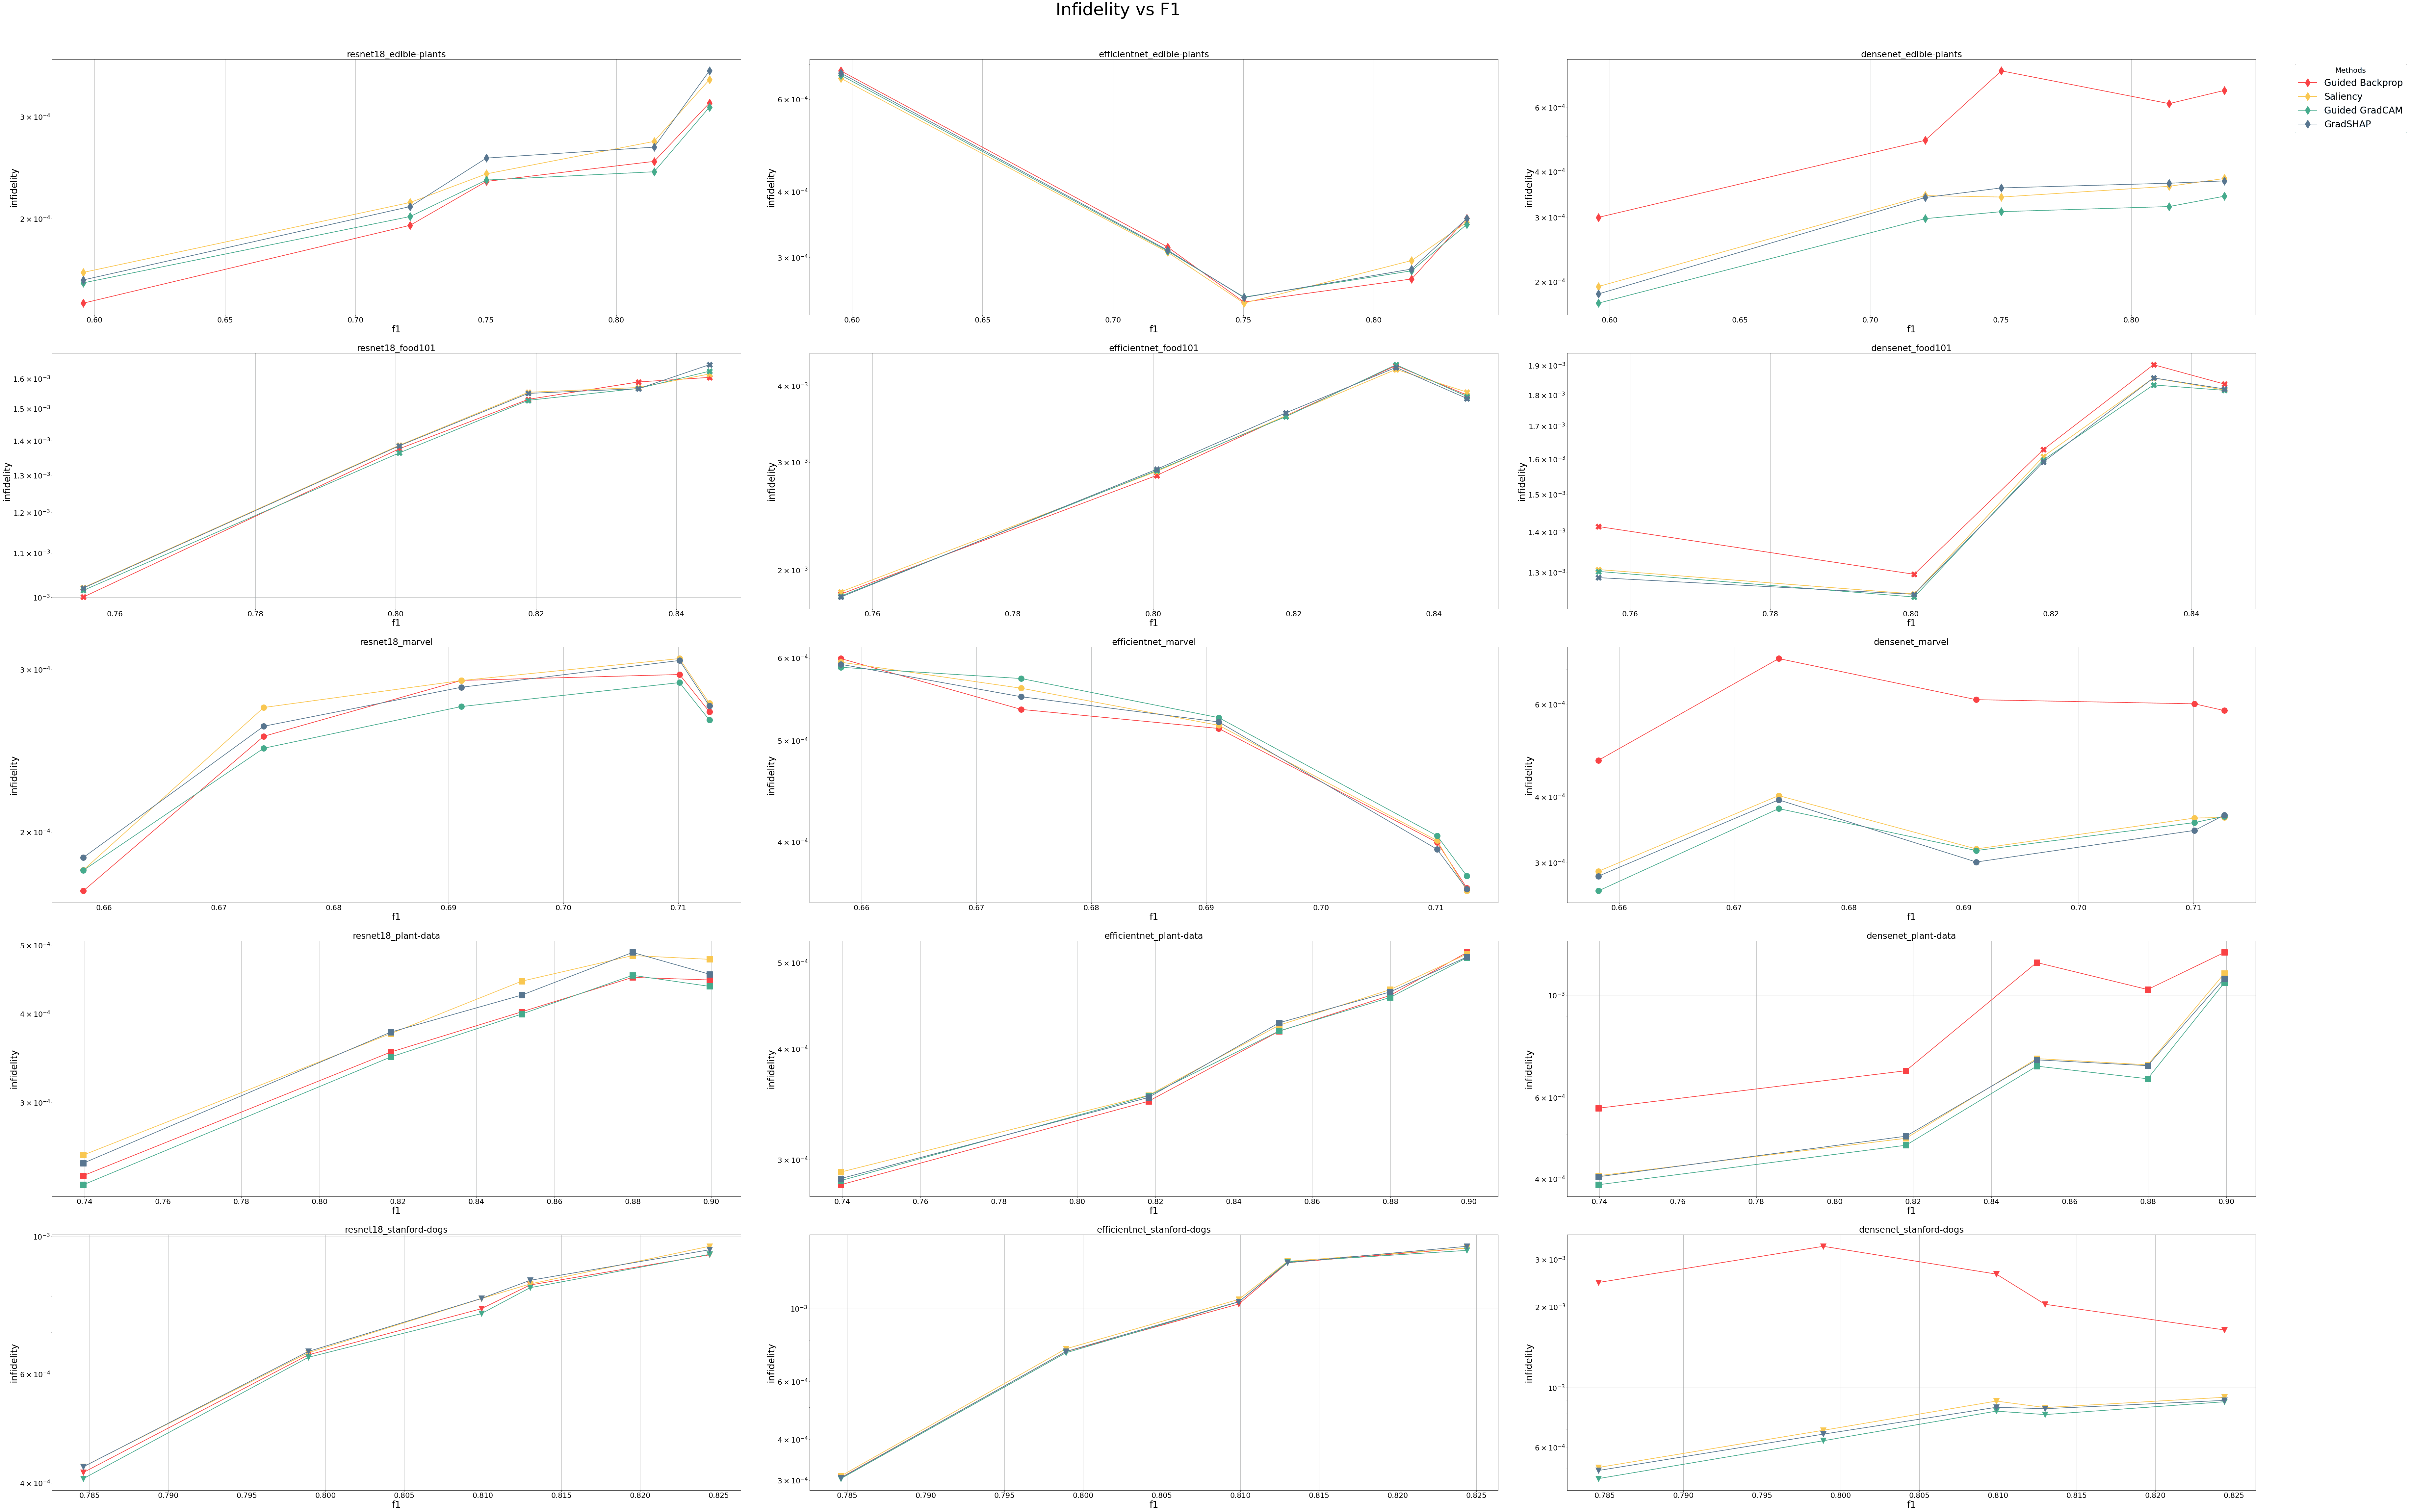
\includegraphics[width=\textwidth]{appendixes/images/inf-combined-f1.png}
  \caption{Combined Infidelity scores against F1 scores. Each row represents a dataset, each column represents an architecture (see individual subplot titles)}\label{fig:combined-infidelity}
\end{figure}

\begin{figure}[ht]
  \centering
    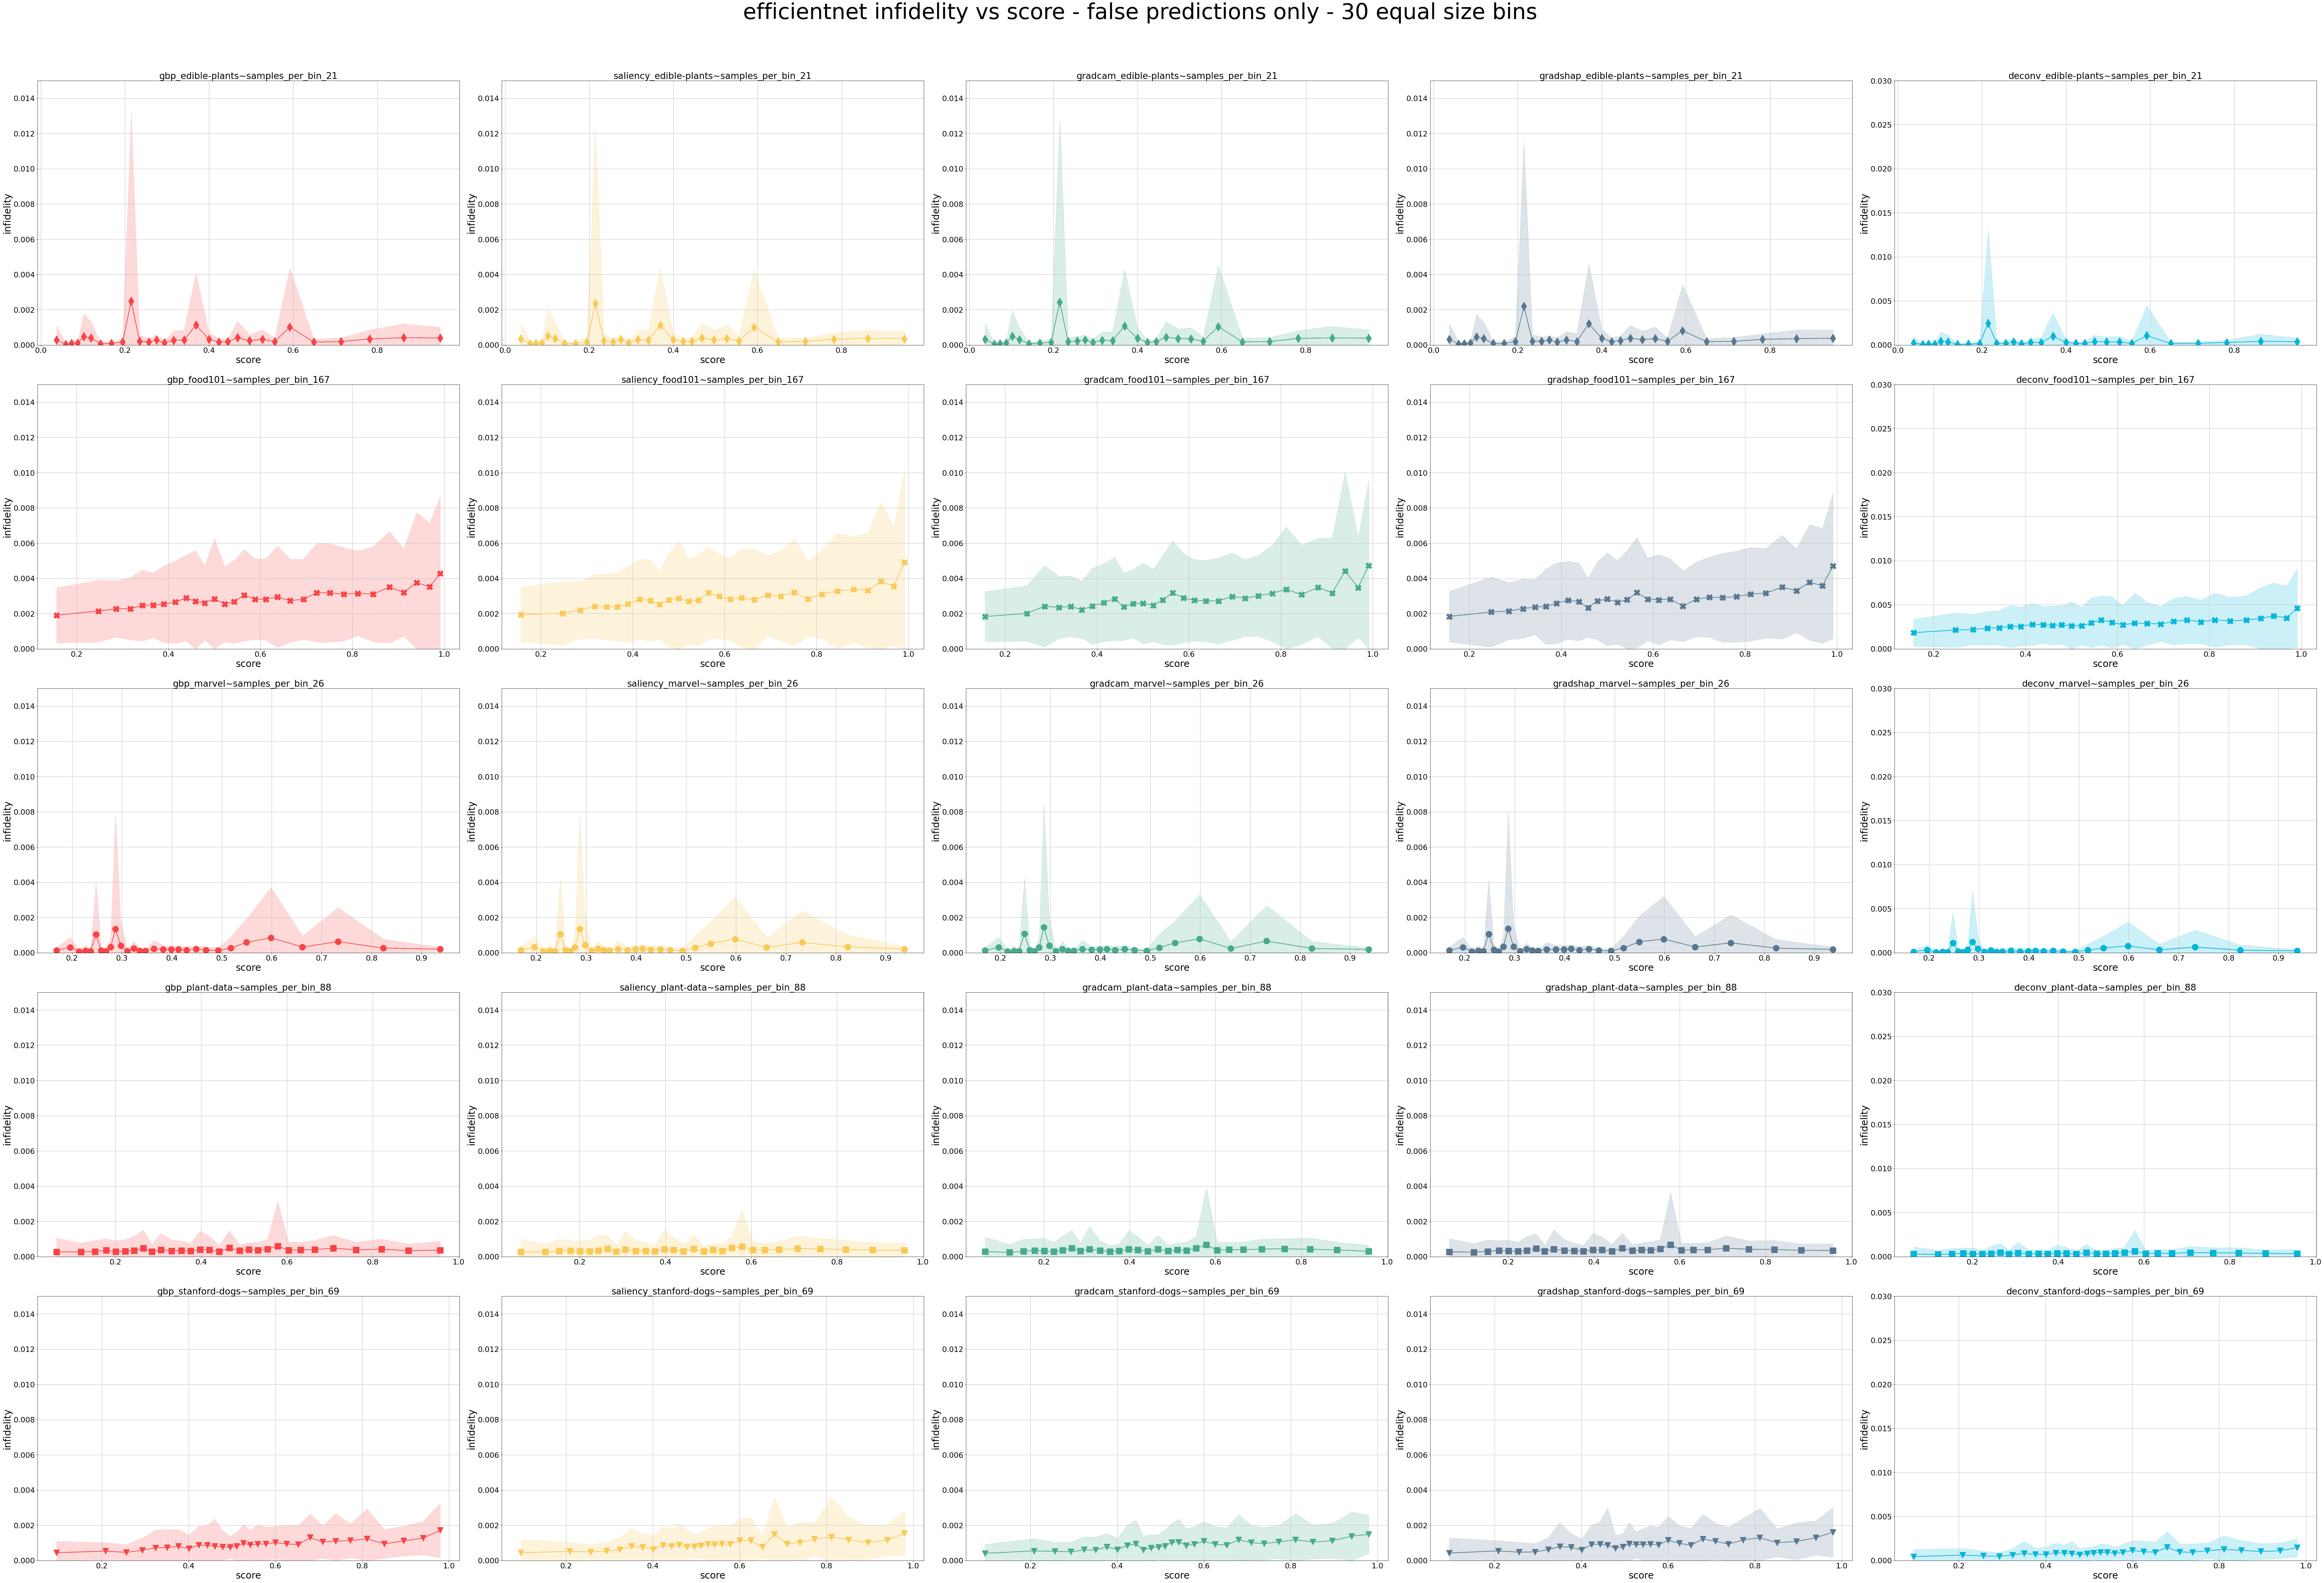
\includegraphics[width=\textwidth]{appendixes/images/efficientnet-infidelity vs score - false predictions only - 30 equal size bins.png}
    \caption{Infidelity scores (with standard deviation) on \textit{EfficientNet B0} architecture. All scores are the mean value for the particular model and are related to that models' predicted scores (x-axis). Each data point is a mean value of the same amount of samples per dataset. Amounts differ between datasets to always split the results into 30 equally-sized bins.}\label{fig:efficientnet-inf-std}
\end{figure}


\begin{figure}[ht]
  \centering
    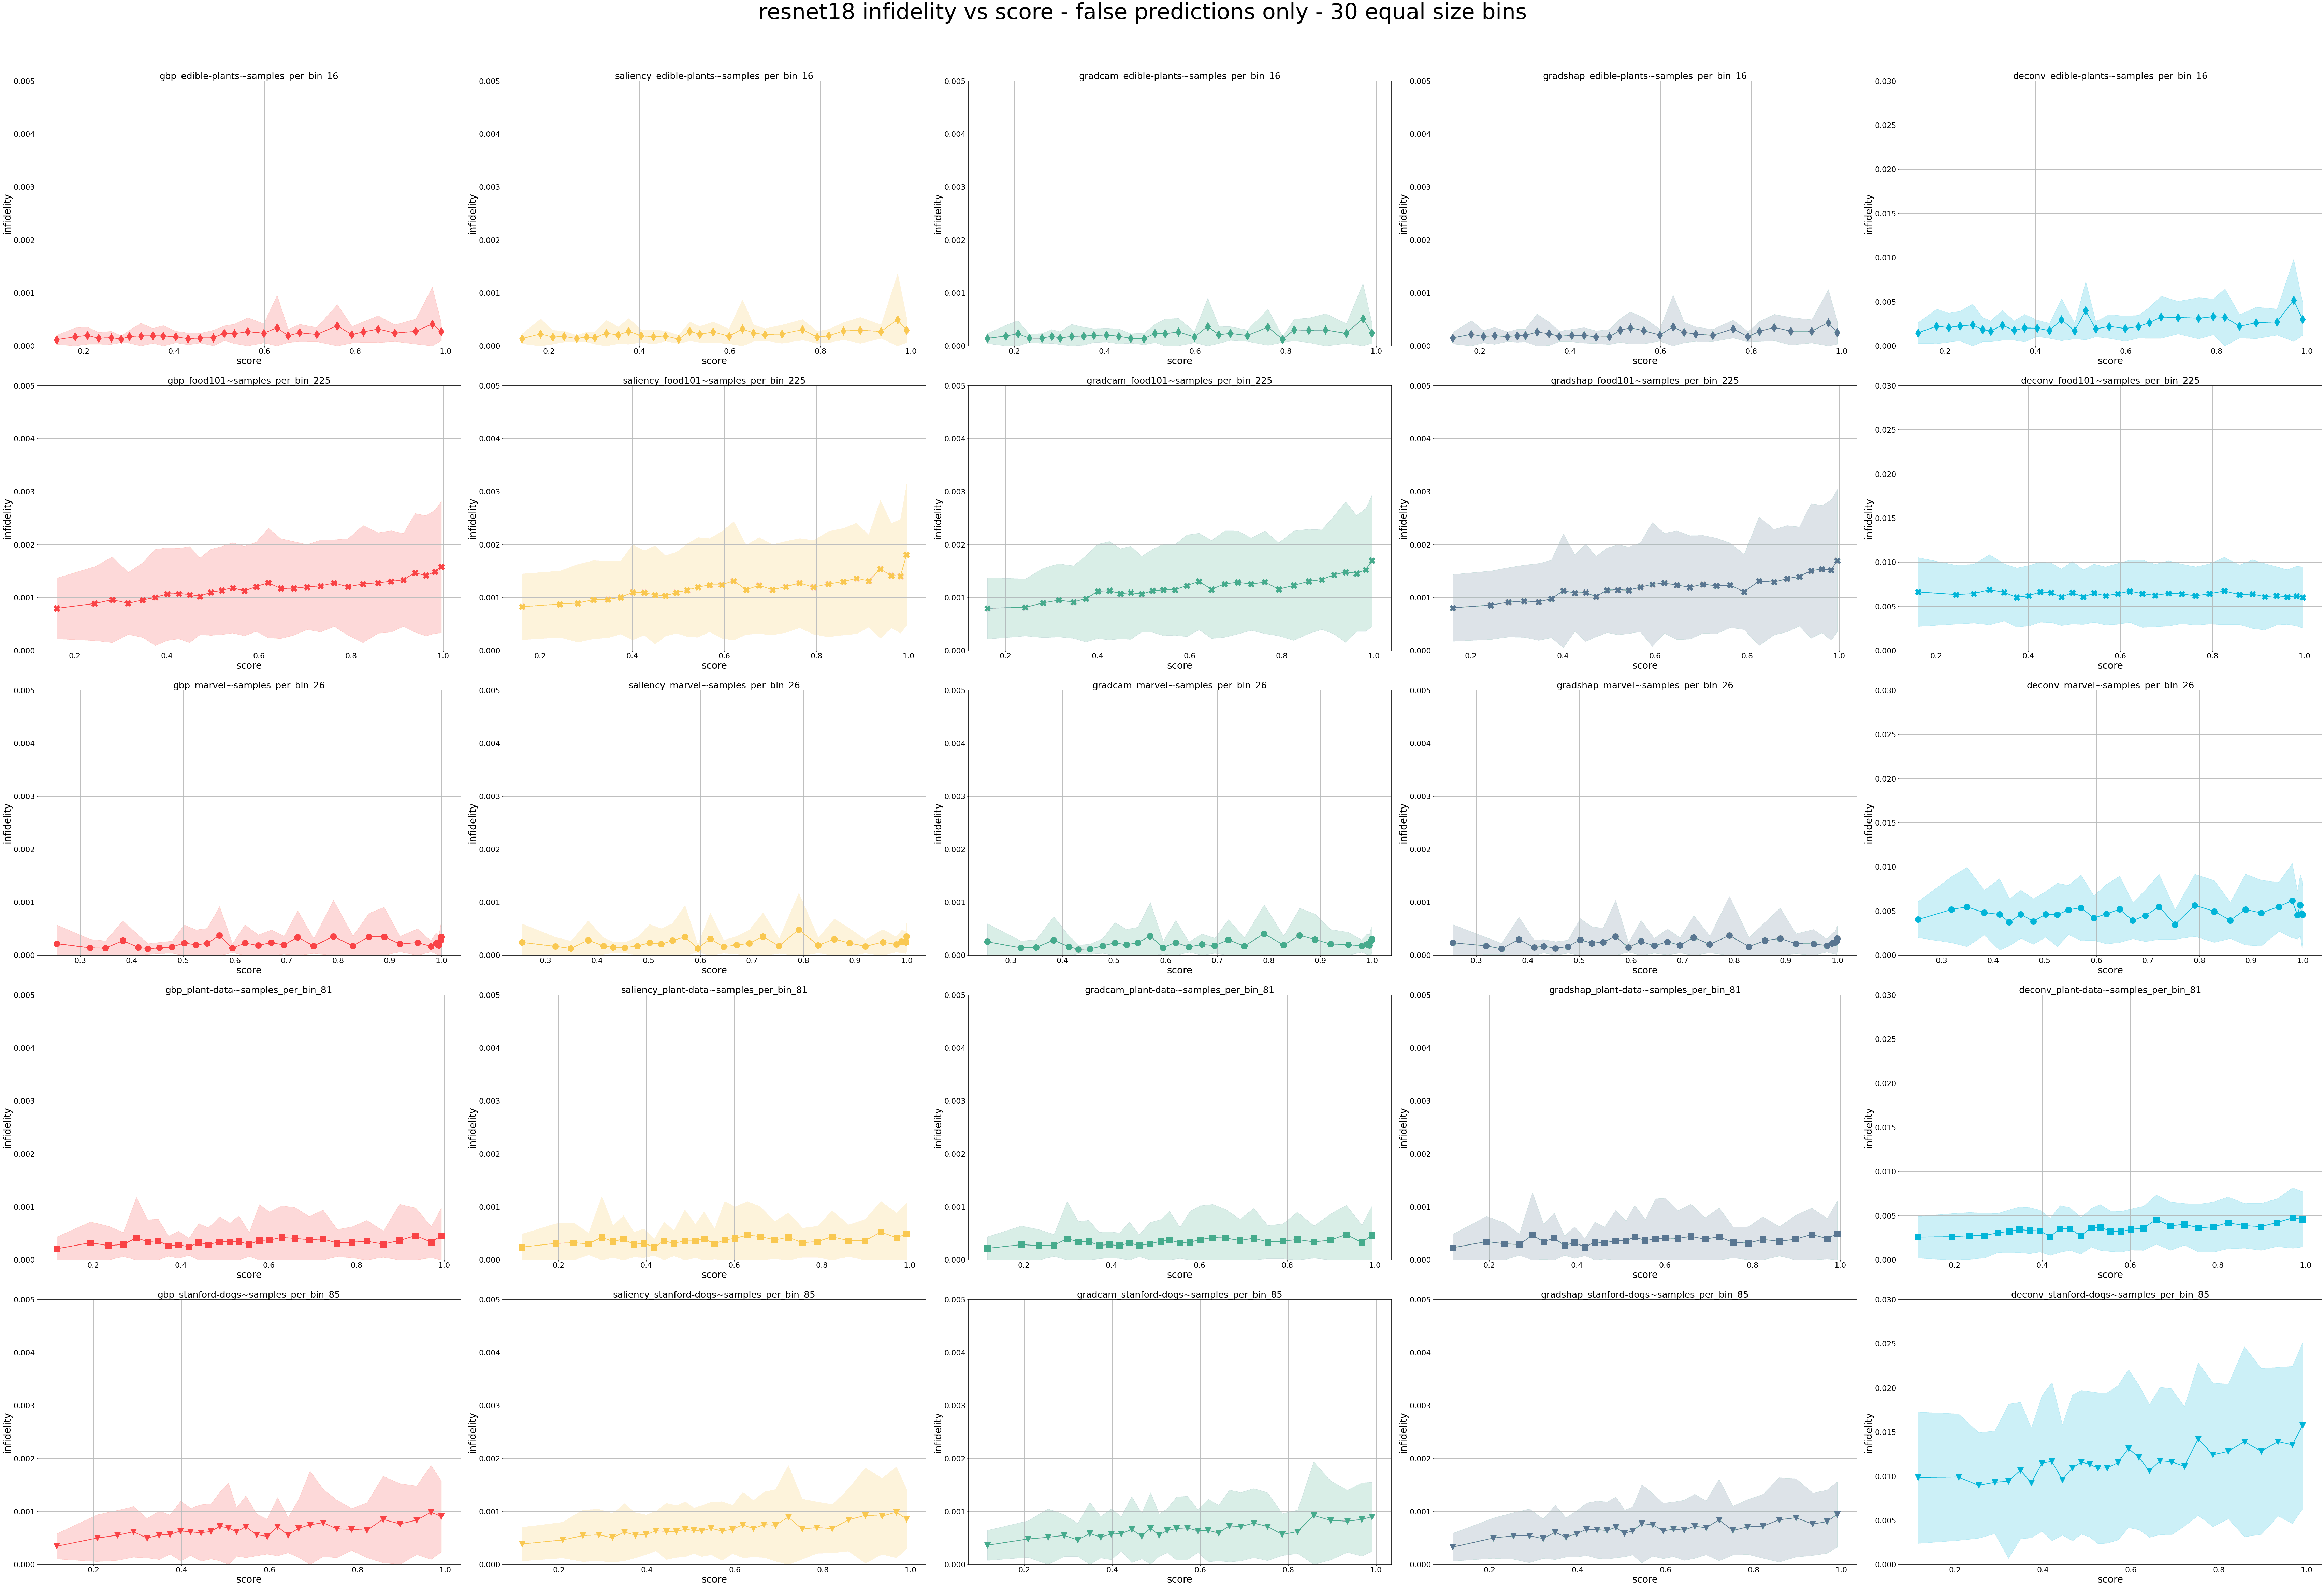
\includegraphics[width=\textwidth]{appendixes/images/resnet18-infidelity vs score - false predictions only - 30 equal size bins.png}
    \caption{Infidelity scores (with standard deviation) on \textit{ResNet18} architecture. All scores are the mean value for the particular model and related to that models' predicted scores (x-axis). Each data point is a meas value of the same amount of samples per dataset. Amounts differ between datasets to always split the results into 30 equally-sized bins.}\label{fig:resnet-inf-std}
\end{figure}

\subsection{Sensitivity - combined scores}\label{appendix:combined-sens}

Individual scores can be find at \url{https://drive.google.com/drive/folders/12eYJSZFMfI2FZhXQSuwJQ6I8w65EU25e?usp=sharing}. Folder "\textbf{individual}" contains separated scores per dataset/model. Folder "\textbf{combined}" contains combined scores. Folder "\textbf{confidence}" contains sensitivity values with standard deviation values.

\begin{figure}[ht]
  \centering
  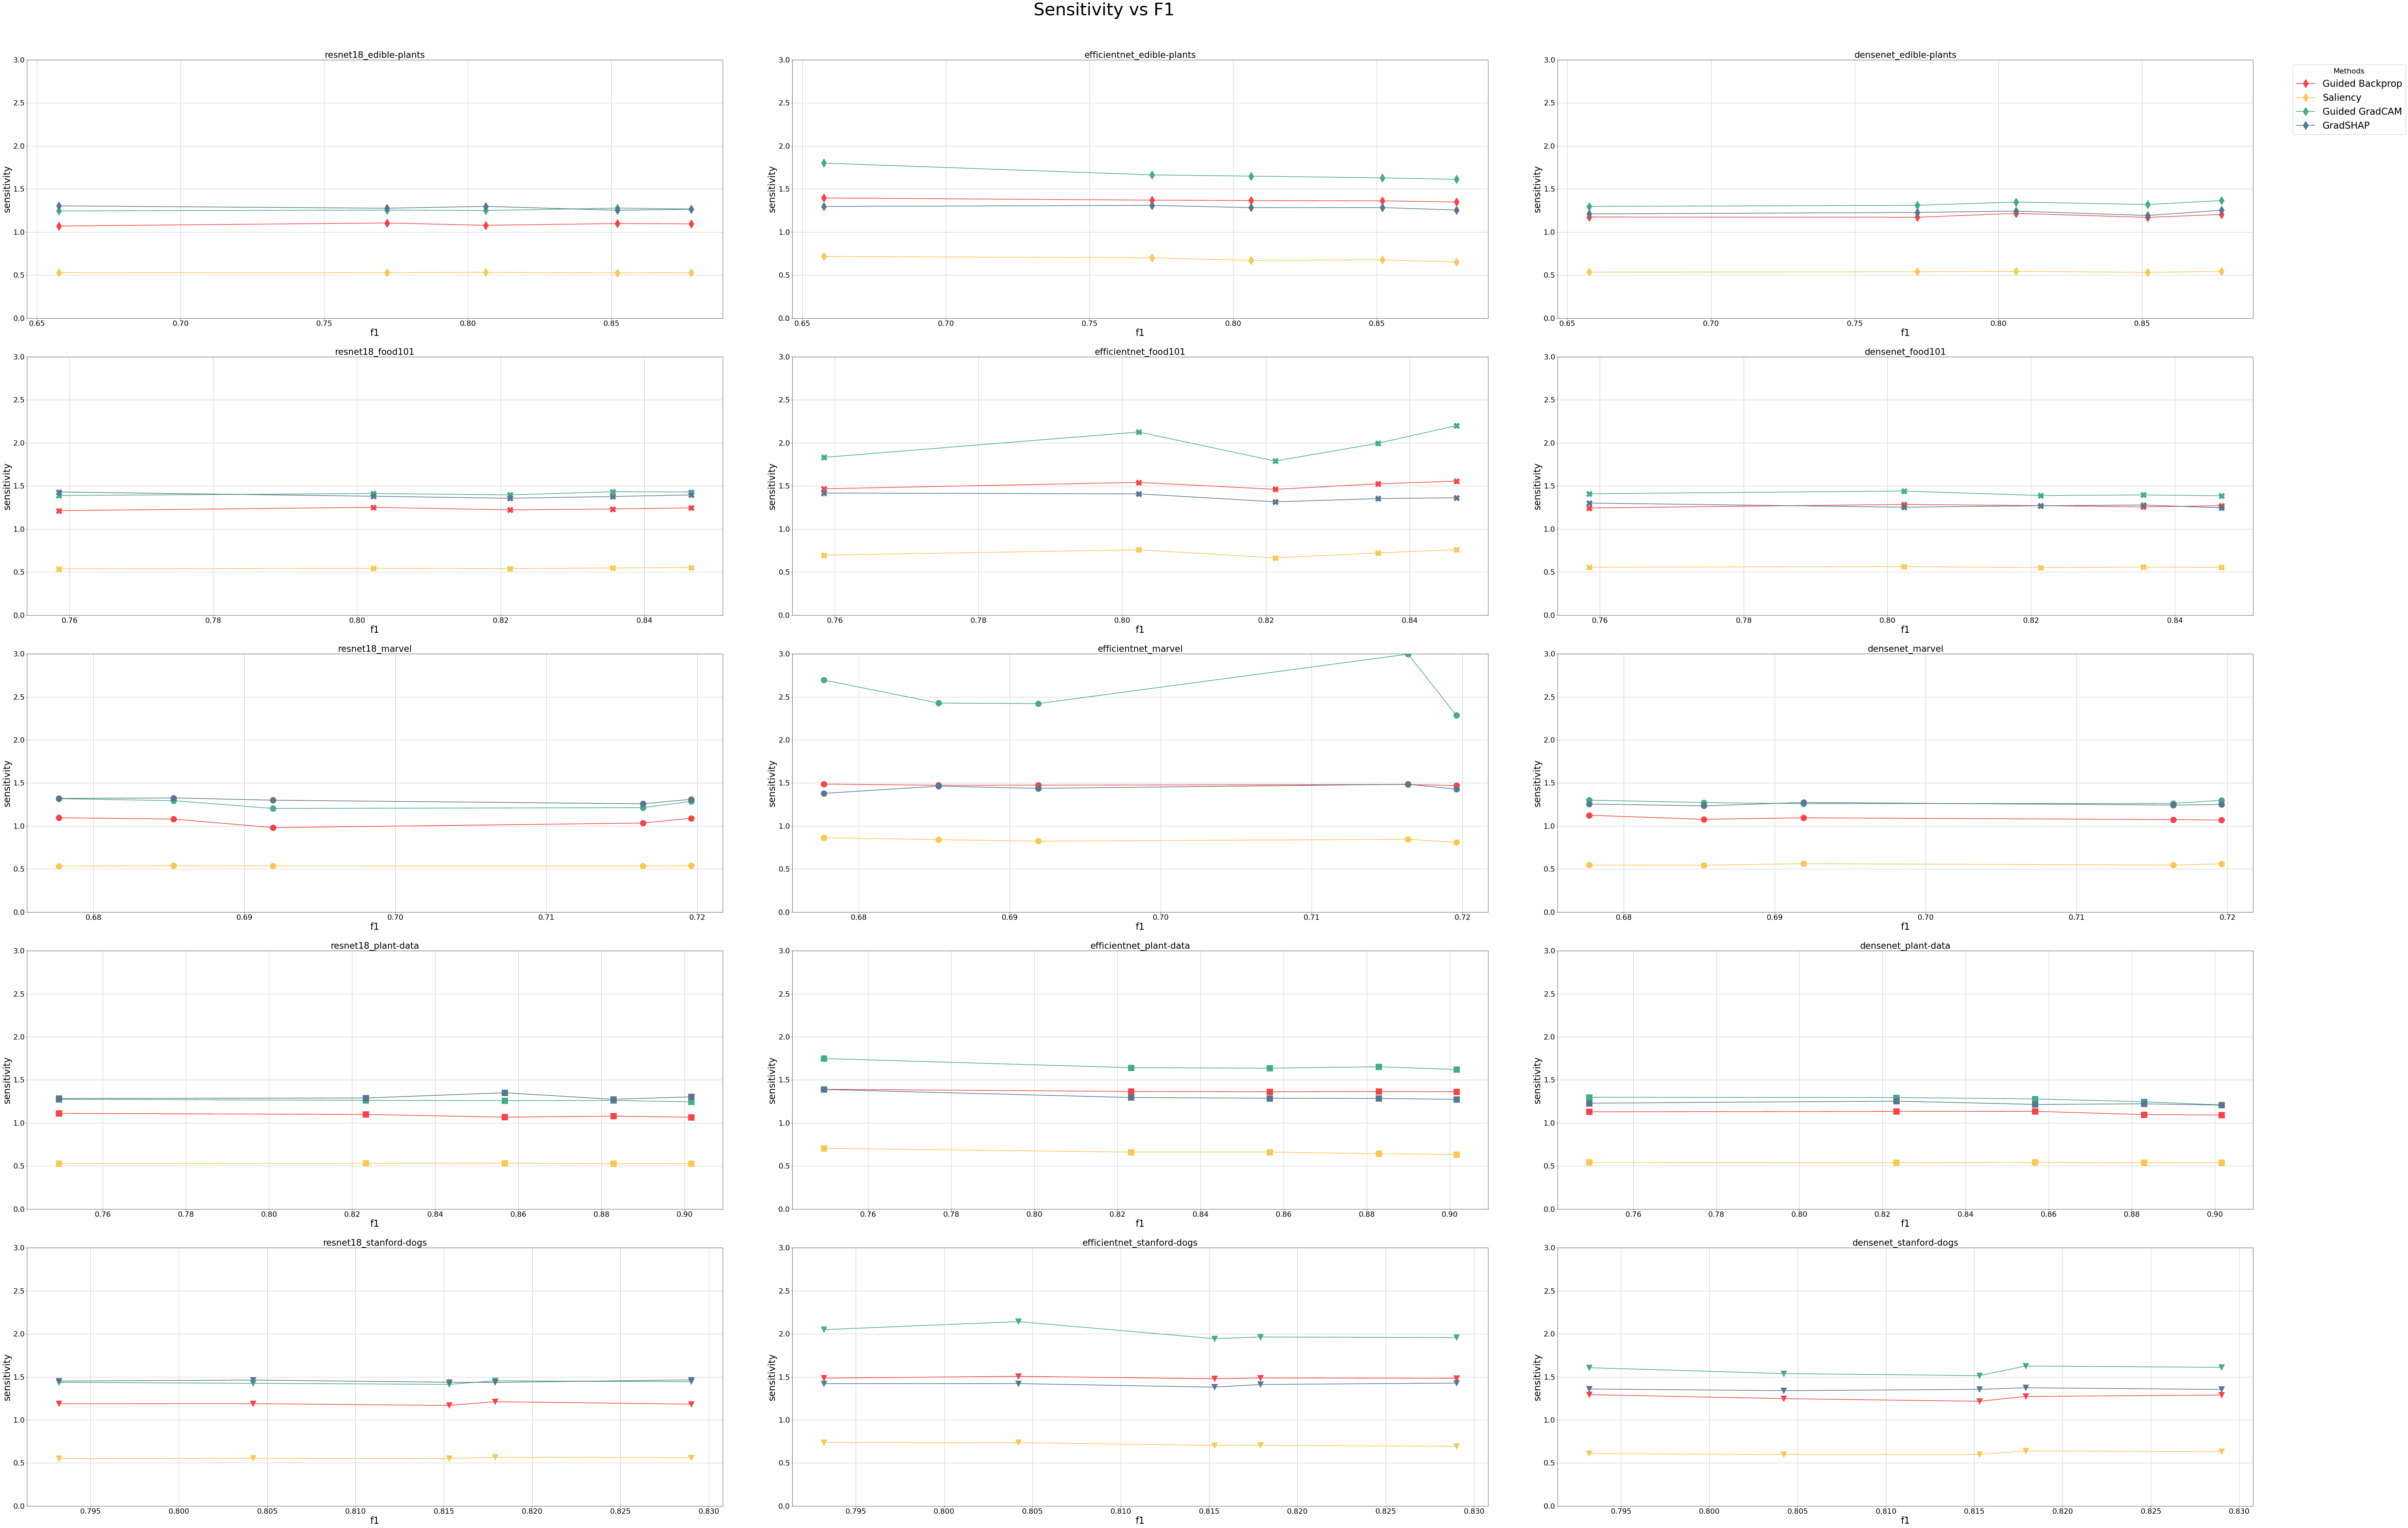
\includegraphics[width=\textwidth]{appendixes/images/sensitivity-combined-f1.png}
  \caption{Combined Sensitivity scores against F1 scores. Each row represents a dataset, each column represents an architecture (see individual subplot titles)}\label{fig:combined-sensitivity}
\end{figure}

\begin{figure}[ht]
  \centering
    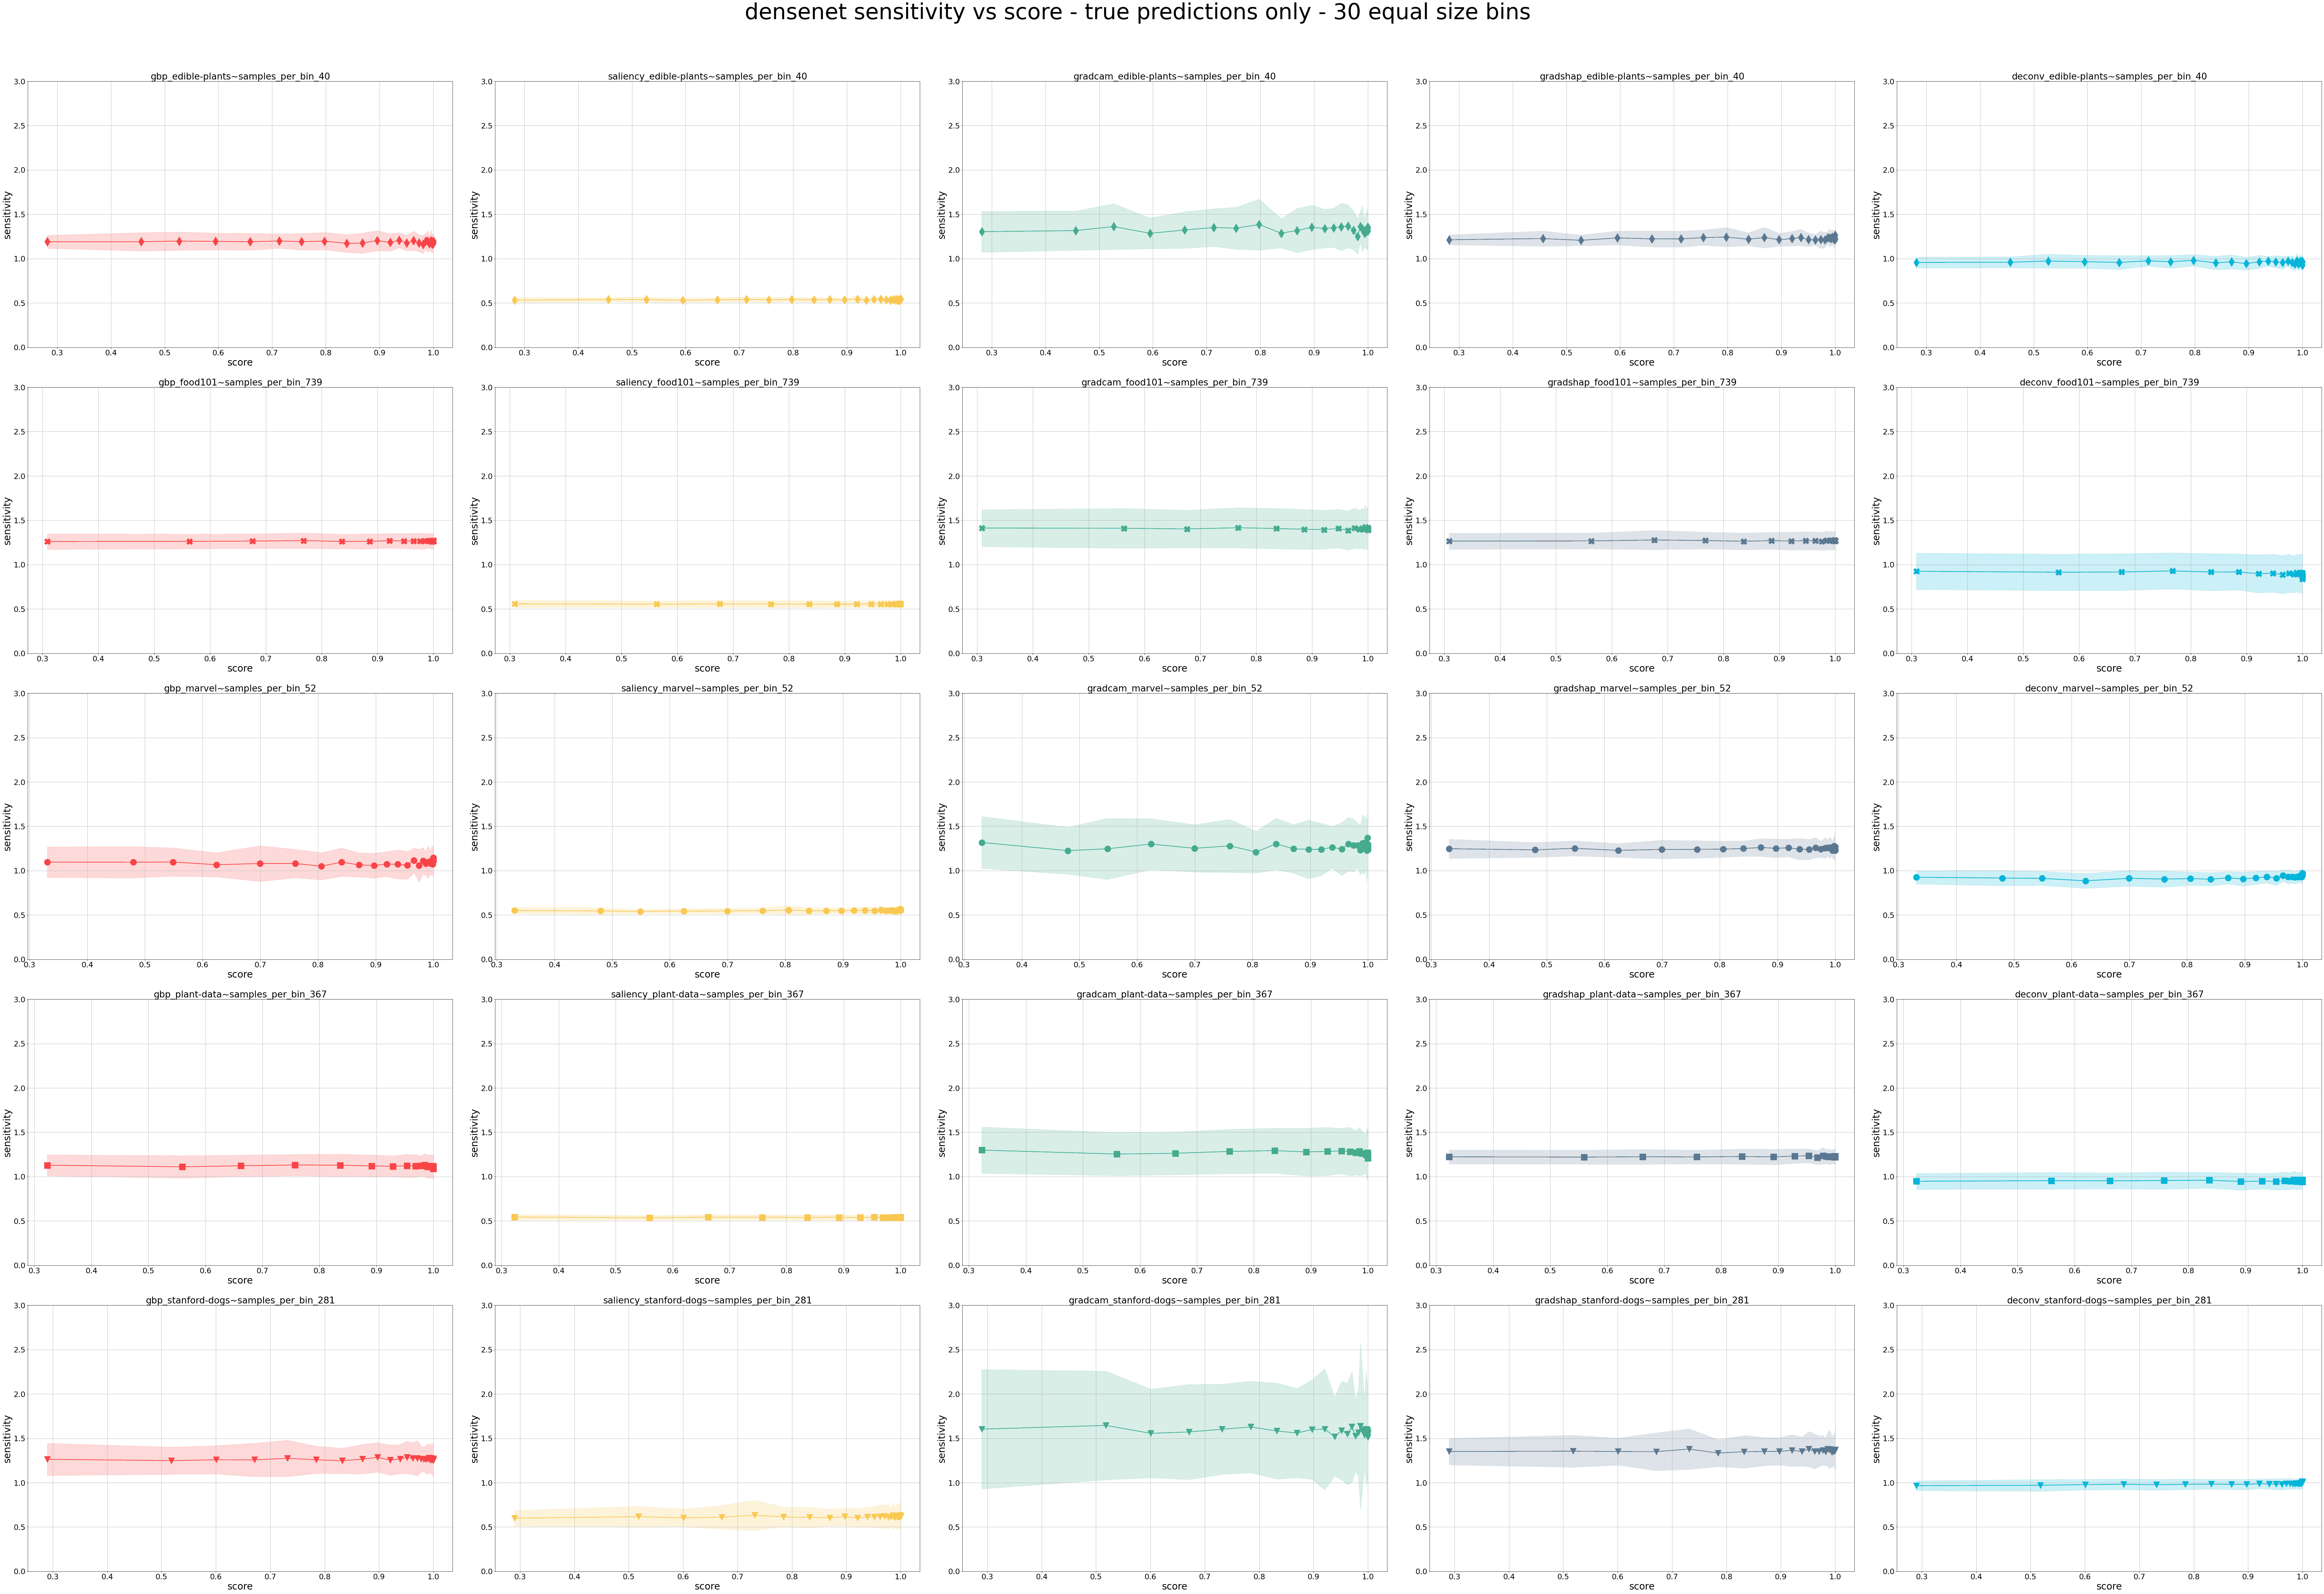
\includegraphics[width=\textwidth]{appendixes/images/densenet-sensitivity vs score - true predictions only - 30 equal size bins.png}
    \caption{Sensitivity scores (with standard deviation) on \textit{DenseNet121} architecture. All scores are the mean value for the particular model and are related to that models' predicted scores (x-axis). Each data point is a mean value of the same amount of samples per dataset. Amounts differ between datasets to always split the results into 30 equally-sized bins.}\label{fig:densenet-sens-std}
\end{figure}